\documentclass{beamer}
\usetheme{Warsaw}
\usepackage{amsmath,amsthm, bm, tikz,qtree,multirow,booktabs}
\usetikzlibrary{arrows,positioning,shapes,fit,calc}
\usepackage[greek,english]{babel}

\title{Probabilistic Forecast Reconciliation}
\date{November 26, 2018}
\author[GPAH]{Puwasala Gamakumara, Anastasios Panagiotelis, George Athanasopoulos and Rob Hyndman}
\begin{document}
  \begin{frame}
    \maketitle
  \end{frame}
  \section{Motivation}
  \begin{frame}{Motivating Examples}
  \begin{itemize}
  	\item Multiple time series $\rightarrow$ some series are aggregates of others.
  	\pause
  	\item Gross Domestic Product \hyperlink{GDP}{\beamerbutton{}}
  	\pause
  	\begin{itemize}
  		\item An aggregate of consumption, investment, government spending and trade balance
  		\item Further breakdown, e.g. consumption of food, rent, etc.
  	\end{itemize}
    \pause
    \item Wind power \hyperlink{aelos}{\beamerbutton{}}
    \begin{itemize}
    	\item Forecasts required at a daily and hourly resolution.
    	\item Daily series is aggregate of 24 hourly series.\label{afterdat}  
    \end{itemize}
    \pause
    \item Potentially need forecasts of all time series.
  \end{itemize}
  \end{frame}
  \begin{frame}{Incoherent Forecasts}
  \begin{itemize}
    \item Potential approaches
    \pause
  	\begin{itemize}
  		\item Multivariate models  		
  		\pause
  		\item Univariate models
  		\pause
  		\item Judgemental forecasts
  	\end{itemize}
  \pause
  \item Forecasts do not respect aggregation structure \pause({\bf Incoherent})\pause
  \item Outcome {\em does} respect aggregation  structure \pause ({\bf Coherent})\pause
  \item Motivation is aggregation but can be generalised to any linear constraints.
  \end{itemize}
  \hfill\hyperlink{bu}{\beamerbutton{}}
  \end{frame}
  \begin{frame}{Reconciliation}\label{cont}
  \begin{itemize}
  	\item Begin with a vector of {\em base} forecasts that are incoherent.
  	\pause
  	\item Adjust these {\bf ex post} to make them coherent.
  	\pause
  	\item There are good solutions for point forecasting that:
  	\pause
  	\begin{itemize}
  		\item Guarantee coherent forecasts.
  		\item Improve forecast accuracy overall.\hfill\hyperlink{macrores}{\beamerbutton{}}
  	\end{itemize}
  	\pause
  	\item Generalisation to probabilistic forecasts is our contribution.
  	\pause
  	\item Getting there necessitates a rethink of the existing point forecasting literature. 
  \end{itemize}
  \end{frame}
%  \begin{frame}{What we do NOT do}
%  \begin{itemize}
%  	\item All information is contained in the most disaggregate series.
%  	\item In principle using the correct multivariate model for the most disaggregate series and aggregating them should work.
%  	\item Disaggregate series are: 
%  	\begin{itemize}
%  		\item Very noisy
%  		\item High-dimensional
%  		\item Prone to model misspecification
%  	\end{itemize} 
%  \end{itemize}
%  \end{frame}
  \section{Point Forecast Reconciliation}
 \begin{frame}{A simple hierarchy}
  	Consider a hierarchy given by
  	\begin{figure}
	    \begin{center}
		\leaf{\alt<2>{\color{blue}AA}{AA}} \leaf{\alt<2>{\color{blue}AB}{AB}} 
		\branch{2}{A}
		\leaf{\alt<2>{\color{blue}BA}{BA}} \leaf{\alt<2>{\color{blue}BB}{BB}}
		\branch{2}{B}
		\branch{2}{Tot}
		\qobitree
	    \end{center}
    \end{figure}
    \begin{itemize}
    	\item Let $n$ be the number of series, $\bm{y}_t$ be an n-vector of all series.
    	\pause\item Let {\color{blue}$m$} be the number of bottom level series and {\color{blue}$\bm{b}_t$} be an {\color{blue}$m$}-vector of the bottom level series.
    \end{itemize}    
\end{frame}  
\begin{frame}{The ${\bm S}$ matrix}
  Coherence holds when
  \begin{equation*}
  {\bm y}_t={\bm S}{\bm b}_t
  \end{equation*} 
    The $n\times m$ matrix ${\bm S}$ defines the aggregation constraints, e.g.
    \begin{equation*}
    {\bm S}=\begin{pmatrix} 1 &1 &1 &1 \\1 &1 &0 &0 \\0 &0 &1 &1 \\ &{\bm I_{4\times 4}}
    \end{pmatrix}  
    \end{equation*}    
\end{frame}
\begin{frame}{As a regression model}
  \begin{itemize}
  	\item Cast the problem as a regression model with base forecasts $\hat{\bm{y}}_{T+h}$ as the ``dependent variable'' and ${\bm S}$ as the ``design matrix''. 
  	\begin{equation*}
  	\hat{\bm{y}}_{T+h}={\bm{S}}{\bm\beta}_{T+h}+{\bm e}_{T+h}
  	\end{equation*}
  	\item Initial approach (Athanasopoulos et al, 2009; Hyndman et al, 2011) was to fit by OLS  yielding reconciled forecasts:
  	\begin{equation*}
  	\tilde{\bm{y}}_{T+h}={\bm S}({\bm S}'{\bm S})^{-1}{\bm S}'{\hat{\bm{y}}}_{T+h}
  	\end{equation*}
  \end{itemize}
\end{frame}
\begin{frame}{Generalisation}
  \begin{itemize}  
  \item Wherever we can use OLS we can use GLS
  \begin{equation*}
  \tilde{\bm{y}}_{T+h}={\bm S}({\bm S}'{\bm W}^{-1}{\bm S})^{-1}{\bm S}'{\bm W}^{-1}{\hat{\bm{y}}}_{T+h}
  \end{equation*}
  \item Diagonal ${\bm W}$ considered by Athanasopoulos et al (2017)
  \item MinT approach (Wickremasuriya et al, 2018) use a ${\bm W}$ that is an estimate of the {\em in-sample} forecast error covariance matrix.
  \end{itemize}
\end{frame}
%  \begin{frame}{Reconciliation in two steps}
%  	\begin{itemize}
%  		\item Many reconciliation methods involve two steps
%  		\begin{enumerate}
%  			\item Pre-multiply $\hat{\bm y}$ by a $m\times n$ matrix $\bm G$ to obtain {\bf bottom} level series ${\bm b}={\bm G}{\hat{\bm y}}$ 
%  			\item Pre-multiply ${\bm b}$ by a $n\times m$ matrix $\bm S$ to obtain ${\tilde{\bm y}}$, i.e. $\tilde{\bm y}={\bm S}{{\bm b}}$
%  		\end{enumerate}
%
%  	    \item Choice of ${\bm G}$ defines reconciliation method, e.g. OLS: ${\bm G}=\left(\bm{S}'\bm{S}\right)^{-1}{\bm S'}$ and Bottom Up: ${\bm G}=\left(\bm{0}_{m\times n-m}~\bm{I}_{m\times m}\right)$ 
%    \end{itemize}
%  \end{frame}
\begin{frame}
\centering
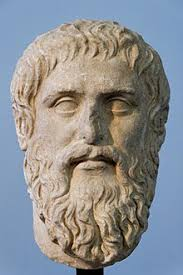
\includegraphics[height=5cm]{Figs/Plato.jpeg}\\
\textgreek{AGEWMTETRHTOS MHDEIS EISITW}\\
Those without knowledge of geometry may not enter.
\end{frame}

  \begin{frame}{Coherent Subspace}
    \begin{definition} 
	  The {\bf coherent subspace} is the $m$-dimensional linear subspace of $\mathbb{R}^n$ spanned by the columns of ${\bm S}$, i.e. $\mathfrak{s}=\mbox{sp}({\bm S})$
    \end{definition}
    Instead of using bottom-level series a different combination of $m$ {\bf basis series} could be used (e.g. top and $m-1$ bottom).\\
    Although ${\bm S}$ would be different $\mathfrak{s}$ would be the same.
  \end{frame}
  \begin{frame}{Coherent Point Forecast}
  \begin{definition} 
  	A {\bf coherent point forecast} is any forecast lying in the linear subspace $\mathfrak{s}$
  \end{definition}
  \end{frame}
  \begin{frame}{Reconciled Point Forecast}
  Let $\hat{\bm y}\in\mathbb{R}^n$ be an incoherent forecast and $g(.)$ be a function $g:\mathbb{R}^n\rightarrow\mathbb{R}^m$.
  \begin{definition} 
	A {\bf point forecast} $\tilde{\bm y}$ is reconciled with respect to $g(.)$ iff 
	\begin{equation*}
    \tilde{\bm y}={\bm S}g(\hat{\bm y})
	\end{equation*}
  \end{definition}
  when $g(.)$ is linear it is easier to write $\tilde{\bm y}={\bm S}{\bm G}\hat{\bm y}$
  \end{frame}
  \begin{frame}{Geometry}
  \vspace{-2.3cm}
  \centering 
  % Created by tikzDevice version 0.11 on 2018-11-10 21:59:53
% !TEX encoding = UTF-8 Unicode
\begin{tikzpicture}[x=0.7pt,y=0.7pt]
\definecolor{fillColor}{RGB}{255,255,255}
\path[use as bounding box,fill=fillColor,fill opacity=0.00] (0,0) rectangle (289.08,505.89);
\begin{scope}
\path[clip] ( 49.20, 61.20) rectangle (263.88,456.69);
\definecolor{drawColor}{RGB}{0,0,0}

\path[draw=drawColor,line width= 0.4pt,line join=round,line cap=round] ( 68.84,106.94) --
	( 68.84,387.57);

\path[draw=drawColor,line width= 0.4pt,line join=round,line cap=round] ( 22.07,153.71) --
	(289.08,153.71);

\path[draw=drawColor,line width= 1.2pt,line join=round,line cap=round] ( 68.84,153.71) -- (232.54,235.56);

\path[draw=drawColor,line width= 1.2pt,line join=round,line cap=round] (222.59,220.48) --
	(232.54,235.56) --
	(214.51,236.64);

\node[text=drawColor,anchor=base west,inner sep=0pt, outer sep=0pt, scale=  1.00] at (238.54,233.26) {{\huge $\mathfrak{s}$}};
\definecolor{drawColor}{RGB}{0,0,255}
\definecolor{fillColor}{RGB}{0,0,255}

\path[draw=drawColor,line width= 0.4pt,line join=round,line cap=round,fill=fillColor] (139.00,294.02) circle (  3.00);
\definecolor{drawColor}{RGB}{0,0,0}

\node[text=drawColor,anchor=base,inner sep=0pt, outer sep=0pt, scale=  1.00] at (139.00,312.02) {{\large $\color{blue}{\hat{\bm{y}}}$}};
\definecolor{drawColor}{RGB}{255,0,0}
\definecolor{fillColor}{RGB}{255,0,0}

\path[draw=drawColor,line width= 0.4pt,line join=round,line cap=round,fill=fillColor] (181.09,209.84) circle (  3.00);
\definecolor{drawColor}{RGB}{0,0,0}

\node[text=drawColor,anchor=base,inner sep=0pt, outer sep=0pt, scale=  1.00] at (181.09,186.10) {{\large $\color{red}{\tilde{\bm{y}}}$}};
\definecolor{drawColor}{RGB}{0,0,255}

\path[draw=drawColor,line width= 0.4pt,line join=round,line cap=round] (139.00,294.02) -- (181.09,209.84);

\path[draw=drawColor,line width= 0.4pt,line join=round,line cap=round] (166.02,219.79) --
	(181.09,209.84) --
	(182.18,227.87);
\definecolor{drawColor}{RGB}{0,0,0}
\definecolor{fillColor}{RGB}{0,0,0}

\path[draw=drawColor,line width= 0.4pt,line join=round,line cap=round,fill=fillColor] (108.93,173.75) circle (  3.00);

\node[text=drawColor,anchor=base,inner sep=0pt, outer sep=0pt, scale=  1.00] at (108.93,150.02) {{\large $\color{black}{{\bm{y}}}$}};
\end{scope}
\end{tikzpicture}

  \end{frame}
%  \begin{frame}{Special Case: Projection}
%  \begin{itemize}
%   \item An important special case is where ${\bm S}{\bm G}$ is a projection.
%  \begin{itemize}
%  	\item ${\bm S}{\bm G}$ is symmetric
%  	\item ${\bm S}{\bm G}$ is idempotent
%  \end{itemize}
%  \item Let ${\bm v}\in\mathfrak{s}$ 
%    \begin{itemize}
%    	\item ${\bm S}{\bm G}{\bm v}$ will also lie in $\mathfrak{s}$.
%    	\item ${\bm S}{\bm G}{\bm v}={\bm v}$ only when ${\bm S}{\bm G}$ is a projection.
%    \end{itemize}
%  \end{itemize}
%  \end{frame}
%
%  \begin{frame}{Geometry: Oblique Projection}
%  	\vspace{-0.9cm}
%  	\centering
%  	% Created by tikzDevice version 0.11 on 2018-04-24 21:50:27
% !TEX encoding = UTF-8 Unicode
\begin{tikzpicture}[x=1pt,y=1pt]
\definecolor{fillColor}{RGB}{255,255,255}
\path[use as bounding box,fill=fillColor,fill opacity=0.00] (0,0) rectangle (505.89,361.35);
\begin{scope}
\path[clip] ( 49.20, 61.20) rectangle (480.69,312.15);
\definecolor{drawColor}{RGB}{0,0,0}

\path[draw=drawColor,line width= 0.4pt,line join=round,line cap=round] ( 88.68, 49.37) --
	( 88.68,302.86);

\path[draw=drawColor,line width= 0.4pt,line join=round,line cap=round] (  0.00, 91.62) --
	(505.89, 91.62);

\path[draw=drawColor,line width= 1.2pt,line join=round,line cap=round] ( 88.68, 91.62) -- (417.71,165.55);

\path[draw=drawColor,line width= 1.2pt,line join=round,line cap=round] (404.42,153.31) --
	(417.71,165.55) --
	(400.46,170.93);

\node[text=drawColor,anchor=base west,inner sep=0pt, outer sep=0pt, scale=  1.00] at (423.71,163.26) {{\Large ${\bm S}$}};

\node[text=drawColor,anchor=base,inner sep=0pt, outer sep=0pt, scale=  1.00] at (276.70,112.53) {{\huge $\mathfrak{s}$}};

\path[draw=drawColor,line width= 1.2pt,line join=round,line cap=round] ( 88.68, 91.62) -- (182.69,260.61);

\path[draw=drawColor,line width= 1.2pt,line join=round,line cap=round] (182.98,242.54) --
	(182.69,260.61) --
	(167.19,251.33);

\node[text=drawColor,anchor=base,inner sep=0pt, outer sep=0pt, scale=  1.00] at (182.69,266.61) {{\Large ${\bm R}$}};

\path[draw=drawColor,line width= 0.4pt,dash pattern=on 4pt off 4pt ,line join=round,line cap=round] (108.22,  0.00) --
	(276.70,302.86);
\definecolor{drawColor}{RGB}{0,0,255}
\definecolor{fillColor}{RGB}{0,0,255}

\path[draw=drawColor,line width= 0.4pt,line join=round,line cap=round,fill=fillColor] (229.69,218.36) circle (  3.00);
\definecolor{drawColor}{RGB}{0,0,0}

\node[text=drawColor,anchor=base,inner sep=0pt, outer sep=0pt, scale=  1.00] at (229.69,236.36) {{\huge $\color{blue}{\hat{\bm{y}}}$}};

\node[text=drawColor,anchor=base west,inner sep=0pt, outer sep=0pt, scale=  1.00] at (212.19,173.82) {{\huge ${\color{blue} s\circ g}$}};
\definecolor{drawColor}{RGB}{255,0,0}
\definecolor{fillColor}{RGB}{255,0,0}

\path[draw=drawColor,line width= 0.4pt,line join=round,line cap=round,fill=fillColor] (169.26,109.72) circle (  3.00);
\definecolor{drawColor}{RGB}{0,0,0}

\node[text=drawColor,anchor=base,inner sep=0pt, outer sep=0pt, scale=  1.00] at (169.26, 85.99) {{\huge $\color{red}{\tilde{\bm{y}}}$}};
\definecolor{drawColor}{RGB}{0,0,255}

\path[draw=drawColor,line width= 0.4pt,line join=round,line cap=round] (229.69,218.36) -- (169.26,109.72);

\path[draw=drawColor,line width= 0.4pt,line join=round,line cap=round] (168.97,127.79) --
	(169.26,109.72) --
	(184.76,119.01);
\end{scope}
\end{tikzpicture}

%  \end{frame}
%  \begin{frame}{Projections preserve unbiasedness}
%	Let $\hat{\bm y}_{t+h|t}$ be an unbiased forecast that is $E_{1:t}(\hat{\bm y}_{t+h|t})={\bm \mu_{t+h|t}}$ where ${\bm \mu_{t+h|t}}=E(\bm{y}_{t+h}\mid\bm{y}_{1},\dots,\bm{y}_{t})$
%	\begin{theorem}
%	  The reconciled forecast $\tilde{\bm y}_{t+h|t}={\bm S}{\bm G}\hat{\bm y}_{t+h|t}$ will also be unbiased iff ${\bm S}{\bm G}$ is a projection.
%    \end{theorem}
%    Previously, this was often stated as an assumption that ${\bm S}{\bm G}{\bm S}={\bm S}$.    
%  \end{frame}
%  \begin{frame}{Proof}
%  Very easy proof
%  \begin{align*}
%  E_{1:t}(\tilde{\bm{y}}_{t+h|t})
%  &= E_{1:t}(\bm{S}\bm{G}\hat{\bm{y}}_{t+h|t})\\
%  &= \bm{S}\bm{G}E_{1:t}(\hat{\bm{y}}_{t+h|t})\\
%  &= \bm{S}\bm{G}\bm{\mu}_{t+h|t}\\
%  &= \bm{\mu}_{t+h|t}
%  \end{align*}
%  The last equality does not hold for ${\bm G}$ in general but does hold when ${\bm S}{\bm G}$ is a projection.
%  \end{frame}
  \begin{frame}{Why reconciliation works}
  \begin{itemize}
  	\item The realised observation always lies on $\mathfrak{s}$.
  	\item Orthogonal projections always get us `closer' to all points in $\mathfrak{s}$ including the actual realisation.
  	\item Ergo reconciliation reduces the error and not just in expectation. 
  	\pause
  	\item What about the MinT approach? 
  \end{itemize}
  \end{frame}
  \begin{frame}{Finding a direction}
  \begin{itemize}
  \item Consider the covariance matrix of ${\bm y}_{T+h}-\hat{\bm{y}}_{T+h}$.
   \pause
   \item This can be estimated using in-sample forecast errors.
   \begin{equation*}
   \bm{W}=\sum\limits_{t=1}^T ({\bm y}_{t}-\hat{\bm{y}}_{t})({\bm y}_{t}-\hat{\bm{y}}_{t})'
   \end{equation*}
  \pause
  \item This provides information about the likely direction of an error.
  \pause
  \item Projecting along this direction is more likely to result in a reconciled forecast that is closer to the target.
  \end{itemize}  
\end{frame}
\begin{frame}{In-Sample errors}
\vspace{-0.9cm}
\centering
% Created by tikzDevice version 0.11 on 2018-11-10 21:59:54
% !TEX encoding = UTF-8 Unicode
\begin{tikzpicture}[x=0.7pt,y=0.7pt]
\definecolor{fillColor}{RGB}{255,255,255}
\path[use as bounding box,fill=fillColor,fill opacity=0.00] (0,0) rectangle (505.89,361.35);
\begin{scope}
\path[clip] ( 49.20, 61.20) rectangle (480.69,312.15);
\definecolor{drawColor}{RGB}{0,0,0}

\path[draw=drawColor,line width= 0.4pt,line join=round,line cap=round] ( 88.68, 49.37) --
	( 88.68,302.86);

\path[draw=drawColor,line width= 0.4pt,line join=round,line cap=round] (  0.00, 91.62) --
	(505.89, 91.62);

\path[draw=drawColor,line width= 1.2pt,line join=round,line cap=round] ( 88.68, 91.62) -- (417.71,165.55);

\path[draw=drawColor,line width= 1.2pt,line join=round,line cap=round] (404.42,153.31) --
	(417.71,165.55) --
	(400.46,170.93);

\node[text=drawColor,anchor=base west,inner sep=0pt, outer sep=0pt, scale=  1.00] at (423.71,163.26) {{\huge $\mathfrak{s}$}};
\definecolor{drawColor}{RGB}{255,165,0}
\definecolor{fillColor}{RGB}{255,165,0}

\path[draw=drawColor,line width= 0.4pt,line join=round,line cap=round,fill=fillColor] ( 80.43, 77.59) circle (  2.25);

\path[draw=drawColor,line width= 0.4pt,line join=round,line cap=round,fill=fillColor] (116.54,119.50) circle (  2.25);

\path[draw=drawColor,line width= 0.4pt,line join=round,line cap=round,fill=fillColor] ( 87.25,127.12) circle (  2.25);

\path[draw=drawColor,line width= 0.4pt,line join=round,line cap=round,fill=fillColor] ( 57.36, 69.82) circle (  2.25);

\path[draw=drawColor,line width= 0.4pt,line join=round,line cap=round,fill=fillColor] (114.20, 90.55) circle (  2.25);

\path[draw=drawColor,line width= 0.4pt,line join=round,line cap=round,fill=fillColor] (131.16,127.97) circle (  2.25);

\path[draw=drawColor,line width= 0.4pt,line join=round,line cap=round,fill=fillColor] ( 88.38,103.67) circle (  2.25);

\path[draw=drawColor,line width= 0.4pt,line join=round,line cap=round,fill=fillColor] ( 96.25, 64.22) circle (  2.25);

\path[draw=drawColor,line width= 0.4pt,line join=round,line cap=round,fill=fillColor] ( 96.58,103.44) circle (  2.25);

\path[draw=drawColor,line width= 0.4pt,line join=round,line cap=round,fill=fillColor] (131.05,195.47) circle (  2.25);

\path[draw=drawColor,line width= 0.4pt,line join=round,line cap=round,fill=fillColor] ( 75.86,123.12) circle (  2.25);

\path[draw=drawColor,line width= 0.4pt,line join=round,line cap=round,fill=fillColor] (101.05, 78.05) circle (  2.25);

\path[draw=drawColor,line width= 0.4pt,line join=round,line cap=round,fill=fillColor] (119.69,170.12) circle (  2.25);

\path[draw=drawColor,line width= 0.4pt,line join=round,line cap=round,fill=fillColor] ( 99.37, 87.87) circle (  2.25);

\path[draw=drawColor,line width= 0.4pt,line join=round,line cap=round,fill=fillColor] ( 90.98, 89.78) circle (  2.25);

\path[draw=drawColor,line width= 0.4pt,line join=round,line cap=round,fill=fillColor] (122.95,161.57) circle (  2.25);

\path[draw=drawColor,line width= 0.4pt,line join=round,line cap=round,fill=fillColor] (118.45, 99.37) circle (  2.25);

\path[draw=drawColor,line width= 0.4pt,line join=round,line cap=round,fill=fillColor] (127.48,131.63) circle (  2.25);

\path[draw=drawColor,line width= 0.4pt,line join=round,line cap=round,fill=fillColor] (118.95,106.61) circle (  2.25);

\path[draw=drawColor,line width= 0.4pt,line join=round,line cap=round,fill=fillColor] ( 78.03, 57.49) circle (  2.25);

\path[draw=drawColor,line width= 0.4pt,line join=round,line cap=round,fill=fillColor] ( 34.47, 51.29) circle (  2.25);

\path[draw=drawColor,line width= 0.4pt,line join=round,line cap=round,fill=fillColor] ( 97.66, 52.97) circle (  2.25);

\path[draw=drawColor,line width= 0.4pt,line join=round,line cap=round,fill=fillColor] ( 70.60, 70.21) circle (  2.25);

\path[draw=drawColor,line width= 0.4pt,line join=round,line cap=round,fill=fillColor] (109.90,140.61) circle (  2.25);

\path[draw=drawColor,line width= 0.4pt,line join=round,line cap=round,fill=fillColor] ( 66.60, 29.73) circle (  2.25);

\path[draw=drawColor,line width= 0.4pt,line join=round,line cap=round,fill=fillColor] (110.40,157.97) circle (  2.25);

\path[draw=drawColor,line width= 0.4pt,line join=round,line cap=round,fill=fillColor] (115.36, 85.61) circle (  2.25);

\path[draw=drawColor,line width= 0.4pt,line join=round,line cap=round,fill=fillColor] ( 67.17, 97.13) circle (  2.25);

\path[draw=drawColor,line width= 0.4pt,line join=round,line cap=round,fill=fillColor] (158.20,202.08) circle (  2.25);

\path[draw=drawColor,line width= 0.4pt,line join=round,line cap=round,fill=fillColor] (127.62,151.92) circle (  2.25);

\path[draw=drawColor,line width= 0.4pt,line join=round,line cap=round,fill=fillColor] (125.07,140.43) circle (  2.25);

\path[draw=drawColor,line width= 0.4pt,line join=round,line cap=round,fill=fillColor] ( 66.95, 79.51) circle (  2.25);

\path[draw=drawColor,line width= 0.4pt,line join=round,line cap=round,fill=fillColor] (159.27,213.20) circle (  2.25);

\path[draw=drawColor,line width= 0.4pt,line join=round,line cap=round,fill=fillColor] (114.76,114.05) circle (  2.25);

\path[draw=drawColor,line width= 0.4pt,line join=round,line cap=round,fill=fillColor] ( 71.40, 91.86) circle (  2.25);

\path[draw=drawColor,line width= 0.4pt,line join=round,line cap=round,fill=fillColor] ( 67.42, 66.76) circle (  2.25);

\path[draw=drawColor,line width= 0.4pt,line join=round,line cap=round,fill=fillColor] (121.31,166.54) circle (  2.25);

\path[draw=drawColor,line width= 0.4pt,line join=round,line cap=round,fill=fillColor] ( 91.87, 84.49) circle (  2.25);

\path[draw=drawColor,line width= 0.4pt,line join=round,line cap=round,fill=fillColor] ( 75.09, 91.11) circle (  2.25);

\path[draw=drawColor,line width= 0.4pt,line join=round,line cap=round,fill=fillColor] ( 50.24, 17.23) circle (  2.25);

\path[draw=drawColor,line width= 0.4pt,line join=round,line cap=round,fill=fillColor] ( 53.96, 95.90) circle (  2.25);

\path[draw=drawColor,line width= 0.4pt,line join=round,line cap=round,fill=fillColor] ( 92.43, 98.29) circle (  2.25);

\path[draw=drawColor,line width= 0.4pt,line join=round,line cap=round,fill=fillColor] (112.78,125.75) circle (  2.25);

\path[draw=drawColor,line width= 0.4pt,line join=round,line cap=round,fill=fillColor] ( 99.39,129.98) circle (  2.25);

\path[draw=drawColor,line width= 0.4pt,line join=round,line cap=round,fill=fillColor] ( 65.81, 67.19) circle (  2.25);

\path[draw=drawColor,line width= 0.4pt,line join=round,line cap=round,fill=fillColor] (165.15,217.44) circle (  2.25);

\path[draw=drawColor,line width= 0.4pt,line join=round,line cap=round,fill=fillColor] (126.47,134.26) circle (  2.25);

\path[draw=drawColor,line width= 0.4pt,line join=round,line cap=round,fill=fillColor] (115.07,130.69) circle (  2.25);

\path[draw=drawColor,line width= 0.4pt,line join=round,line cap=round,fill=fillColor] ( 82.26, 74.72) circle (  2.25);

\path[draw=drawColor,line width= 0.4pt,line join=round,line cap=round,fill=fillColor] ( 86.20, 53.43) circle (  2.25);

\path[draw=drawColor,line width= 0.4pt,line join=round,line cap=round,fill=fillColor] (101.58, 77.11) circle (  2.25);

\path[draw=drawColor,line width= 0.4pt,line join=round,line cap=round,fill=fillColor] ( 74.66, 49.18) circle (  2.25);

\path[draw=drawColor,line width= 0.4pt,line join=round,line cap=round,fill=fillColor] ( 80.49, 53.85) circle (  2.25);

\path[draw=drawColor,line width= 0.4pt,line join=round,line cap=round,fill=fillColor] ( 59.74, 16.50) circle (  2.25);

\path[draw=drawColor,line width= 0.4pt,line join=round,line cap=round,fill=fillColor] ( 88.11, 68.83) circle (  2.25);

\path[draw=drawColor,line width= 0.4pt,line join=round,line cap=round,fill=fillColor] (118.66,124.73) circle (  2.25);

\path[draw=drawColor,line width= 0.4pt,line join=round,line cap=round,fill=fillColor] ( 62.31, 37.48) circle (  2.25);

\path[draw=drawColor,line width= 0.4pt,line join=round,line cap=round,fill=fillColor] ( 61.74, 72.76) circle (  2.25);

\path[draw=drawColor,line width= 0.4pt,line join=round,line cap=round,fill=fillColor] ( 61.11, 76.99) circle (  2.25);

\path[draw=drawColor,line width= 0.4pt,line join=round,line cap=round,fill=fillColor] (128.45,175.85) circle (  2.25);

\path[draw=drawColor,line width= 0.4pt,line join=round,line cap=round,fill=fillColor] ( 85.40,108.73) circle (  2.25);

\path[draw=drawColor,line width= 0.4pt,line join=round,line cap=round,fill=fillColor] (155.00,162.51) circle (  2.25);

\path[draw=drawColor,line width= 0.4pt,line join=round,line cap=round,fill=fillColor] ( 51.21, 58.57) circle (  2.25);

\path[draw=drawColor,line width= 0.4pt,line join=round,line cap=round,fill=fillColor] ( 61.02, 49.15) circle (  2.25);

\path[draw=drawColor,line width= 0.4pt,line join=round,line cap=round,fill=fillColor] ( 97.00, 98.42) circle (  2.25);

\path[draw=drawColor,line width= 0.4pt,line join=round,line cap=round,fill=fillColor] ( 78.51,112.39) circle (  2.25);

\path[draw=drawColor,line width= 0.4pt,line join=round,line cap=round,fill=fillColor] ( 74.09, 80.07) circle (  2.25);

\path[draw=drawColor,line width= 0.4pt,line join=round,line cap=round,fill=fillColor] ( 88.80, 96.98) circle (  2.25);

\path[draw=drawColor,line width= 0.4pt,line join=round,line cap=round,fill=fillColor] (115.15,114.86) circle (  2.25);

\path[draw=drawColor,line width= 0.4pt,line join=round,line cap=round,fill=fillColor] ( 86.11, 73.34) circle (  2.25);

\path[draw=drawColor,line width= 0.4pt,line join=round,line cap=round,fill=fillColor] ( 80.06, 12.45) circle (  2.25);

\path[draw=drawColor,line width= 0.4pt,line join=round,line cap=round,fill=fillColor] (107.35, 72.84) circle (  2.25);

\path[draw=drawColor,line width= 0.4pt,line join=round,line cap=round,fill=fillColor] (112.38,134.67) circle (  2.25);

\path[draw=drawColor,line width= 0.4pt,line join=round,line cap=round,fill=fillColor] (127.15,137.80) circle (  2.25);

\path[draw=drawColor,line width= 0.4pt,line join=round,line cap=round,fill=fillColor] ( 84.24, 77.30) circle (  2.25);

\path[draw=drawColor,line width= 0.4pt,line join=round,line cap=round,fill=fillColor] ( 66.51, 28.94) circle (  2.25);

\path[draw=drawColor,line width= 0.4pt,line join=round,line cap=round,fill=fillColor] ( 37.32, 67.95) circle (  2.25);

\path[draw=drawColor,line width= 0.4pt,line join=round,line cap=round,fill=fillColor] (101.26,132.62) circle (  2.25);

\path[draw=drawColor,line width= 0.4pt,line join=round,line cap=round,fill=fillColor] (113.47,107.08) circle (  2.25);

\path[draw=drawColor,line width= 0.4pt,line join=round,line cap=round,fill=fillColor] ( 91.84, 73.01) circle (  2.25);

\path[draw=drawColor,line width= 0.4pt,line join=round,line cap=round,fill=fillColor] (108.94,155.81) circle (  2.25);

\path[draw=drawColor,line width= 0.4pt,line join=round,line cap=round,fill=fillColor] ( 95.18, 98.18) circle (  2.25);

\path[draw=drawColor,line width= 0.4pt,line join=round,line cap=round,fill=fillColor] (117.18,161.11) circle (  2.25);

\path[draw=drawColor,line width= 0.4pt,line join=round,line cap=round,fill=fillColor] ( 95.76, 73.23) circle (  2.25);

\path[draw=drawColor,line width= 0.4pt,line join=round,line cap=round,fill=fillColor] (112.56,107.96) circle (  2.25);

\path[draw=drawColor,line width= 0.4pt,line join=round,line cap=round,fill=fillColor] ( 72.77, 70.07) circle (  2.25);

\path[draw=drawColor,line width= 0.4pt,line join=round,line cap=round,fill=fillColor] ( 59.67,101.13) circle (  2.25);

\path[draw=drawColor,line width= 0.4pt,line join=round,line cap=round,fill=fillColor] ( 83.94, 84.86) circle (  2.25);

\path[draw=drawColor,line width= 0.4pt,line join=round,line cap=round,fill=fillColor] ( 74.70, 45.01) circle (  2.25);

\path[draw=drawColor,line width= 0.4pt,line join=round,line cap=round,fill=fillColor] (111.65, 95.16) circle (  2.25);

\path[draw=drawColor,line width= 0.4pt,line join=round,line cap=round,fill=fillColor] ( 60.12, 44.38) circle (  2.25);

\path[draw=drawColor,line width= 0.4pt,line join=round,line cap=round,fill=fillColor] ( 84.85, 58.30) circle (  2.25);

\path[draw=drawColor,line width= 0.4pt,line join=round,line cap=round,fill=fillColor] ( 80.98, 82.39) circle (  2.25);

\path[draw=drawColor,line width= 0.4pt,line join=round,line cap=round,fill=fillColor] (115.59,136.74) circle (  2.25);

\path[draw=drawColor,line width= 0.4pt,line join=round,line cap=round,fill=fillColor] ( 85.06, 76.31) circle (  2.25);

\path[draw=drawColor,line width= 0.4pt,line join=round,line cap=round,fill=fillColor] ( 90.25, 59.16) circle (  2.25);

\path[draw=drawColor,line width= 0.4pt,line join=round,line cap=round,fill=fillColor] ( 62.80, 53.18) circle (  2.25);

\path[draw=drawColor,line width= 0.4pt,line join=round,line cap=round,fill=fillColor] (146.14,197.55) circle (  2.25);
\end{scope}
\end{tikzpicture}

\end{frame}
\begin{frame}{Most likely direction}
\vspace{-0.9cm}
\centering
% Created by tikzDevice version 0.11 on 2018-11-10 21:59:54
% !TEX encoding = UTF-8 Unicode
\begin{tikzpicture}[x=0.7pt,y=0.7pt]
\definecolor{fillColor}{RGB}{255,255,255}
\path[use as bounding box,fill=fillColor,fill opacity=0.00] (0,0) rectangle (505.89,361.35);
\begin{scope}
\path[clip] ( 49.20, 61.20) rectangle (480.69,312.15);
\definecolor{drawColor}{RGB}{0,0,0}

\path[draw=drawColor,line width= 0.4pt,line join=round,line cap=round] ( 88.68, 49.37) --
	( 88.68,302.86);

\path[draw=drawColor,line width= 0.4pt,line join=round,line cap=round] (  0.00, 91.62) --
	(505.89, 91.62);

\path[draw=drawColor,line width= 1.2pt,line join=round,line cap=round] ( 88.68, 91.62) -- (417.71,165.55);

\path[draw=drawColor,line width= 1.2pt,line join=round,line cap=round] (404.42,153.31) --
	(417.71,165.55) --
	(400.46,170.93);

\node[text=drawColor,anchor=base west,inner sep=0pt, outer sep=0pt, scale=  1.00] at (423.71,163.26) {{\huge $\mathfrak{s}$}};
\definecolor{drawColor}{RGB}{255,165,0}
\definecolor{fillColor}{RGB}{255,165,0}

\path[draw=drawColor,line width= 0.4pt,line join=round,line cap=round,fill=fillColor] ( 80.43, 77.59) circle (  2.25);

\path[draw=drawColor,line width= 0.4pt,line join=round,line cap=round,fill=fillColor] (116.54,119.50) circle (  2.25);

\path[draw=drawColor,line width= 0.4pt,line join=round,line cap=round,fill=fillColor] ( 87.25,127.12) circle (  2.25);

\path[draw=drawColor,line width= 0.4pt,line join=round,line cap=round,fill=fillColor] ( 57.36, 69.82) circle (  2.25);

\path[draw=drawColor,line width= 0.4pt,line join=round,line cap=round,fill=fillColor] (114.20, 90.55) circle (  2.25);

\path[draw=drawColor,line width= 0.4pt,line join=round,line cap=round,fill=fillColor] (131.16,127.97) circle (  2.25);

\path[draw=drawColor,line width= 0.4pt,line join=round,line cap=round,fill=fillColor] ( 88.38,103.67) circle (  2.25);

\path[draw=drawColor,line width= 0.4pt,line join=round,line cap=round,fill=fillColor] ( 96.25, 64.22) circle (  2.25);

\path[draw=drawColor,line width= 0.4pt,line join=round,line cap=round,fill=fillColor] ( 96.58,103.44) circle (  2.25);

\path[draw=drawColor,line width= 0.4pt,line join=round,line cap=round,fill=fillColor] (131.05,195.47) circle (  2.25);

\path[draw=drawColor,line width= 0.4pt,line join=round,line cap=round,fill=fillColor] ( 75.86,123.12) circle (  2.25);

\path[draw=drawColor,line width= 0.4pt,line join=round,line cap=round,fill=fillColor] (101.05, 78.05) circle (  2.25);

\path[draw=drawColor,line width= 0.4pt,line join=round,line cap=round,fill=fillColor] (119.69,170.12) circle (  2.25);

\path[draw=drawColor,line width= 0.4pt,line join=round,line cap=round,fill=fillColor] ( 99.37, 87.87) circle (  2.25);

\path[draw=drawColor,line width= 0.4pt,line join=round,line cap=round,fill=fillColor] ( 90.98, 89.78) circle (  2.25);

\path[draw=drawColor,line width= 0.4pt,line join=round,line cap=round,fill=fillColor] (122.95,161.57) circle (  2.25);

\path[draw=drawColor,line width= 0.4pt,line join=round,line cap=round,fill=fillColor] (118.45, 99.37) circle (  2.25);

\path[draw=drawColor,line width= 0.4pt,line join=round,line cap=round,fill=fillColor] (127.48,131.63) circle (  2.25);

\path[draw=drawColor,line width= 0.4pt,line join=round,line cap=round,fill=fillColor] (118.95,106.61) circle (  2.25);

\path[draw=drawColor,line width= 0.4pt,line join=round,line cap=round,fill=fillColor] ( 78.03, 57.49) circle (  2.25);

\path[draw=drawColor,line width= 0.4pt,line join=round,line cap=round,fill=fillColor] ( 34.47, 51.29) circle (  2.25);

\path[draw=drawColor,line width= 0.4pt,line join=round,line cap=round,fill=fillColor] ( 97.66, 52.97) circle (  2.25);

\path[draw=drawColor,line width= 0.4pt,line join=round,line cap=round,fill=fillColor] ( 70.60, 70.21) circle (  2.25);

\path[draw=drawColor,line width= 0.4pt,line join=round,line cap=round,fill=fillColor] (109.90,140.61) circle (  2.25);

\path[draw=drawColor,line width= 0.4pt,line join=round,line cap=round,fill=fillColor] ( 66.60, 29.73) circle (  2.25);

\path[draw=drawColor,line width= 0.4pt,line join=round,line cap=round,fill=fillColor] (110.40,157.97) circle (  2.25);

\path[draw=drawColor,line width= 0.4pt,line join=round,line cap=round,fill=fillColor] (115.36, 85.61) circle (  2.25);

\path[draw=drawColor,line width= 0.4pt,line join=round,line cap=round,fill=fillColor] ( 67.17, 97.13) circle (  2.25);

\path[draw=drawColor,line width= 0.4pt,line join=round,line cap=round,fill=fillColor] (158.20,202.08) circle (  2.25);

\path[draw=drawColor,line width= 0.4pt,line join=round,line cap=round,fill=fillColor] (127.62,151.92) circle (  2.25);

\path[draw=drawColor,line width= 0.4pt,line join=round,line cap=round,fill=fillColor] (125.07,140.43) circle (  2.25);

\path[draw=drawColor,line width= 0.4pt,line join=round,line cap=round,fill=fillColor] ( 66.95, 79.51) circle (  2.25);

\path[draw=drawColor,line width= 0.4pt,line join=round,line cap=round,fill=fillColor] (159.27,213.20) circle (  2.25);

\path[draw=drawColor,line width= 0.4pt,line join=round,line cap=round,fill=fillColor] (114.76,114.05) circle (  2.25);

\path[draw=drawColor,line width= 0.4pt,line join=round,line cap=round,fill=fillColor] ( 71.40, 91.86) circle (  2.25);

\path[draw=drawColor,line width= 0.4pt,line join=round,line cap=round,fill=fillColor] ( 67.42, 66.76) circle (  2.25);

\path[draw=drawColor,line width= 0.4pt,line join=round,line cap=round,fill=fillColor] (121.31,166.54) circle (  2.25);

\path[draw=drawColor,line width= 0.4pt,line join=round,line cap=round,fill=fillColor] ( 91.87, 84.49) circle (  2.25);

\path[draw=drawColor,line width= 0.4pt,line join=round,line cap=round,fill=fillColor] ( 75.09, 91.11) circle (  2.25);

\path[draw=drawColor,line width= 0.4pt,line join=round,line cap=round,fill=fillColor] ( 50.24, 17.23) circle (  2.25);

\path[draw=drawColor,line width= 0.4pt,line join=round,line cap=round,fill=fillColor] ( 53.96, 95.90) circle (  2.25);

\path[draw=drawColor,line width= 0.4pt,line join=round,line cap=round,fill=fillColor] ( 92.43, 98.29) circle (  2.25);

\path[draw=drawColor,line width= 0.4pt,line join=round,line cap=round,fill=fillColor] (112.78,125.75) circle (  2.25);

\path[draw=drawColor,line width= 0.4pt,line join=round,line cap=round,fill=fillColor] ( 99.39,129.98) circle (  2.25);

\path[draw=drawColor,line width= 0.4pt,line join=round,line cap=round,fill=fillColor] ( 65.81, 67.19) circle (  2.25);

\path[draw=drawColor,line width= 0.4pt,line join=round,line cap=round,fill=fillColor] (165.15,217.44) circle (  2.25);

\path[draw=drawColor,line width= 0.4pt,line join=round,line cap=round,fill=fillColor] (126.47,134.26) circle (  2.25);

\path[draw=drawColor,line width= 0.4pt,line join=round,line cap=round,fill=fillColor] (115.07,130.69) circle (  2.25);

\path[draw=drawColor,line width= 0.4pt,line join=round,line cap=round,fill=fillColor] ( 82.26, 74.72) circle (  2.25);

\path[draw=drawColor,line width= 0.4pt,line join=round,line cap=round,fill=fillColor] ( 86.20, 53.43) circle (  2.25);

\path[draw=drawColor,line width= 0.4pt,line join=round,line cap=round,fill=fillColor] (101.58, 77.11) circle (  2.25);

\path[draw=drawColor,line width= 0.4pt,line join=round,line cap=round,fill=fillColor] ( 74.66, 49.18) circle (  2.25);

\path[draw=drawColor,line width= 0.4pt,line join=round,line cap=round,fill=fillColor] ( 80.49, 53.85) circle (  2.25);

\path[draw=drawColor,line width= 0.4pt,line join=round,line cap=round,fill=fillColor] ( 59.74, 16.50) circle (  2.25);

\path[draw=drawColor,line width= 0.4pt,line join=round,line cap=round,fill=fillColor] ( 88.11, 68.83) circle (  2.25);

\path[draw=drawColor,line width= 0.4pt,line join=round,line cap=round,fill=fillColor] (118.66,124.73) circle (  2.25);

\path[draw=drawColor,line width= 0.4pt,line join=round,line cap=round,fill=fillColor] ( 62.31, 37.48) circle (  2.25);

\path[draw=drawColor,line width= 0.4pt,line join=round,line cap=round,fill=fillColor] ( 61.74, 72.76) circle (  2.25);

\path[draw=drawColor,line width= 0.4pt,line join=round,line cap=round,fill=fillColor] ( 61.11, 76.99) circle (  2.25);

\path[draw=drawColor,line width= 0.4pt,line join=round,line cap=round,fill=fillColor] (128.45,175.85) circle (  2.25);

\path[draw=drawColor,line width= 0.4pt,line join=round,line cap=round,fill=fillColor] ( 85.40,108.73) circle (  2.25);

\path[draw=drawColor,line width= 0.4pt,line join=round,line cap=round,fill=fillColor] (155.00,162.51) circle (  2.25);

\path[draw=drawColor,line width= 0.4pt,line join=round,line cap=round,fill=fillColor] ( 51.21, 58.57) circle (  2.25);

\path[draw=drawColor,line width= 0.4pt,line join=round,line cap=round,fill=fillColor] ( 61.02, 49.15) circle (  2.25);

\path[draw=drawColor,line width= 0.4pt,line join=round,line cap=round,fill=fillColor] ( 97.00, 98.42) circle (  2.25);

\path[draw=drawColor,line width= 0.4pt,line join=round,line cap=round,fill=fillColor] ( 78.51,112.39) circle (  2.25);

\path[draw=drawColor,line width= 0.4pt,line join=round,line cap=round,fill=fillColor] ( 74.09, 80.07) circle (  2.25);

\path[draw=drawColor,line width= 0.4pt,line join=round,line cap=round,fill=fillColor] ( 88.80, 96.98) circle (  2.25);

\path[draw=drawColor,line width= 0.4pt,line join=round,line cap=round,fill=fillColor] (115.15,114.86) circle (  2.25);

\path[draw=drawColor,line width= 0.4pt,line join=round,line cap=round,fill=fillColor] ( 86.11, 73.34) circle (  2.25);

\path[draw=drawColor,line width= 0.4pt,line join=round,line cap=round,fill=fillColor] ( 80.06, 12.45) circle (  2.25);

\path[draw=drawColor,line width= 0.4pt,line join=round,line cap=round,fill=fillColor] (107.35, 72.84) circle (  2.25);

\path[draw=drawColor,line width= 0.4pt,line join=round,line cap=round,fill=fillColor] (112.38,134.67) circle (  2.25);

\path[draw=drawColor,line width= 0.4pt,line join=round,line cap=round,fill=fillColor] (127.15,137.80) circle (  2.25);

\path[draw=drawColor,line width= 0.4pt,line join=round,line cap=round,fill=fillColor] ( 84.24, 77.30) circle (  2.25);

\path[draw=drawColor,line width= 0.4pt,line join=round,line cap=round,fill=fillColor] ( 66.51, 28.94) circle (  2.25);

\path[draw=drawColor,line width= 0.4pt,line join=round,line cap=round,fill=fillColor] ( 37.32, 67.95) circle (  2.25);

\path[draw=drawColor,line width= 0.4pt,line join=round,line cap=round,fill=fillColor] (101.26,132.62) circle (  2.25);

\path[draw=drawColor,line width= 0.4pt,line join=round,line cap=round,fill=fillColor] (113.47,107.08) circle (  2.25);

\path[draw=drawColor,line width= 0.4pt,line join=round,line cap=round,fill=fillColor] ( 91.84, 73.01) circle (  2.25);

\path[draw=drawColor,line width= 0.4pt,line join=round,line cap=round,fill=fillColor] (108.94,155.81) circle (  2.25);

\path[draw=drawColor,line width= 0.4pt,line join=round,line cap=round,fill=fillColor] ( 95.18, 98.18) circle (  2.25);

\path[draw=drawColor,line width= 0.4pt,line join=round,line cap=round,fill=fillColor] (117.18,161.11) circle (  2.25);

\path[draw=drawColor,line width= 0.4pt,line join=round,line cap=round,fill=fillColor] ( 95.76, 73.23) circle (  2.25);

\path[draw=drawColor,line width= 0.4pt,line join=round,line cap=round,fill=fillColor] (112.56,107.96) circle (  2.25);

\path[draw=drawColor,line width= 0.4pt,line join=round,line cap=round,fill=fillColor] ( 72.77, 70.07) circle (  2.25);

\path[draw=drawColor,line width= 0.4pt,line join=round,line cap=round,fill=fillColor] ( 59.67,101.13) circle (  2.25);

\path[draw=drawColor,line width= 0.4pt,line join=round,line cap=round,fill=fillColor] ( 83.94, 84.86) circle (  2.25);

\path[draw=drawColor,line width= 0.4pt,line join=round,line cap=round,fill=fillColor] ( 74.70, 45.01) circle (  2.25);

\path[draw=drawColor,line width= 0.4pt,line join=round,line cap=round,fill=fillColor] (111.65, 95.16) circle (  2.25);

\path[draw=drawColor,line width= 0.4pt,line join=round,line cap=round,fill=fillColor] ( 60.12, 44.38) circle (  2.25);

\path[draw=drawColor,line width= 0.4pt,line join=round,line cap=round,fill=fillColor] ( 84.85, 58.30) circle (  2.25);

\path[draw=drawColor,line width= 0.4pt,line join=round,line cap=round,fill=fillColor] ( 80.98, 82.39) circle (  2.25);

\path[draw=drawColor,line width= 0.4pt,line join=round,line cap=round,fill=fillColor] (115.59,136.74) circle (  2.25);

\path[draw=drawColor,line width= 0.4pt,line join=round,line cap=round,fill=fillColor] ( 85.06, 76.31) circle (  2.25);

\path[draw=drawColor,line width= 0.4pt,line join=round,line cap=round,fill=fillColor] ( 90.25, 59.16) circle (  2.25);

\path[draw=drawColor,line width= 0.4pt,line join=round,line cap=round,fill=fillColor] ( 62.80, 53.18) circle (  2.25);

\path[draw=drawColor,line width= 0.4pt,line join=round,line cap=round,fill=fillColor] (146.14,197.55) circle (  2.25);
\definecolor{drawColor}{RGB}{0,0,0}

\path[draw=drawColor,line width= 1.2pt,line join=round,line cap=round] ( 88.68, 91.62) -- (182.69,260.61);

\path[draw=drawColor,line width= 1.2pt,line join=round,line cap=round] (182.98,242.54) --
	(182.69,260.61) --
	(167.19,251.33);

\node[text=drawColor,anchor=base,inner sep=0pt, outer sep=0pt, scale=  1.00] at (182.69,266.61) {{\Large ${\bm R}$}};
\end{scope}
\end{tikzpicture}

\end{frame}
  \begin{frame}{Geometry: Oblique Projection}
\vspace{-0.9cm}
\centering
% Created by tikzDevice version 0.11 on 2018-11-10 21:59:54
% !TEX encoding = UTF-8 Unicode
\begin{tikzpicture}[x=0.7pt,y=0.7pt]
\definecolor{fillColor}{RGB}{255,255,255}
\path[use as bounding box,fill=fillColor,fill opacity=0.00] (0,0) rectangle (505.89,361.35);
\begin{scope}
\path[clip] ( 49.20, 61.20) rectangle (480.69,312.15);
\definecolor{drawColor}{RGB}{0,0,0}

\path[draw=drawColor,line width= 0.4pt,line join=round,line cap=round] ( 88.68, 49.37) --
	( 88.68,302.86);

\path[draw=drawColor,line width= 0.4pt,line join=round,line cap=round] (  0.00, 91.62) --
	(505.89, 91.62);

\path[draw=drawColor,line width= 1.2pt,line join=round,line cap=round] ( 88.68, 91.62) -- (417.71,165.55);

\path[draw=drawColor,line width= 1.2pt,line join=round,line cap=round] (404.42,153.31) --
	(417.71,165.55) --
	(400.46,170.93);

\node[text=drawColor,anchor=base west,inner sep=0pt, outer sep=0pt, scale=  1.00] at (423.71,163.26) {{\huge $\mathfrak{s}$}};

\path[draw=drawColor,line width= 1.2pt,line join=round,line cap=round] ( 88.68, 91.62) -- (182.69,260.61);

\path[draw=drawColor,line width= 1.2pt,line join=round,line cap=round] (182.98,242.54) --
	(182.69,260.61) --
	(167.19,251.33);

\node[text=drawColor,anchor=base,inner sep=0pt, outer sep=0pt, scale=  1.00] at (182.69,266.61) {{\Large ${\bm R}$}};
\definecolor{fillColor}{RGB}{0,0,0}

\path[draw=drawColor,line width= 0.4pt,line join=round,line cap=round,fill=fillColor] (145.09,104.29) circle (  3.00);

\node[text=drawColor,anchor=base,inner sep=0pt, outer sep=0pt, scale=  1.00] at (145.09, 86.55) {{\huge $\color{black}{\bm{y}}$}};
\end{scope}
\end{tikzpicture}

\end{frame}
  \begin{frame}{Geometry: Oblique Projection}
\vspace{-0.9cm}
\centering
% Created by tikzDevice version 0.11 on 2018-11-10 21:59:54
% !TEX encoding = UTF-8 Unicode
\begin{tikzpicture}[x=0.7pt,y=0.7pt]
\definecolor{fillColor}{RGB}{255,255,255}
\path[use as bounding box,fill=fillColor,fill opacity=0.00] (0,0) rectangle (505.89,361.35);
\begin{scope}
\path[clip] ( 49.20, 61.20) rectangle (480.69,312.15);
\definecolor{drawColor}{RGB}{0,0,0}

\path[draw=drawColor,line width= 0.4pt,line join=round,line cap=round] ( 88.68, 49.37) --
	( 88.68,302.86);

\path[draw=drawColor,line width= 0.4pt,line join=round,line cap=round] (  0.00, 91.62) --
	(505.89, 91.62);
\definecolor{drawColor}{RGB}{190,190,190}
\definecolor{fillColor}{RGB}{190,190,190}

\path[draw=drawColor,line width= 0.4pt,line join=round,line cap=round,fill=fillColor] (136.83, 90.26) circle (  2.25);

\path[draw=drawColor,line width= 0.4pt,line join=round,line cap=round,fill=fillColor] (172.94,132.17) circle (  2.25);

\path[draw=drawColor,line width= 0.4pt,line join=round,line cap=round,fill=fillColor] (143.65,139.79) circle (  2.25);

\path[draw=drawColor,line width= 0.4pt,line join=round,line cap=round,fill=fillColor] (113.76, 82.49) circle (  2.25);

\path[draw=drawColor,line width= 0.4pt,line join=round,line cap=round,fill=fillColor] (170.60,103.23) circle (  2.25);

\path[draw=drawColor,line width= 0.4pt,line join=round,line cap=round,fill=fillColor] (187.56,140.65) circle (  2.25);

\path[draw=drawColor,line width= 0.4pt,line join=round,line cap=round,fill=fillColor] (144.79,116.34) circle (  2.25);

\path[draw=drawColor,line width= 0.4pt,line join=round,line cap=round,fill=fillColor] (152.65, 76.89) circle (  2.25);

\path[draw=drawColor,line width= 0.4pt,line join=round,line cap=round,fill=fillColor] (152.98,116.12) circle (  2.25);

\path[draw=drawColor,line width= 0.4pt,line join=round,line cap=round,fill=fillColor] (187.45,208.14) circle (  2.25);

\path[draw=drawColor,line width= 0.4pt,line join=round,line cap=round,fill=fillColor] (132.26,135.79) circle (  2.25);

\path[draw=drawColor,line width= 0.4pt,line join=round,line cap=round,fill=fillColor] (157.45, 90.72) circle (  2.25);

\path[draw=drawColor,line width= 0.4pt,line join=round,line cap=round,fill=fillColor] (176.09,182.79) circle (  2.25);

\path[draw=drawColor,line width= 0.4pt,line join=round,line cap=round,fill=fillColor] (155.77,100.54) circle (  2.25);

\path[draw=drawColor,line width= 0.4pt,line join=round,line cap=round,fill=fillColor] (147.38,102.45) circle (  2.25);

\path[draw=drawColor,line width= 0.4pt,line join=round,line cap=round,fill=fillColor] (179.36,174.24) circle (  2.25);

\path[draw=drawColor,line width= 0.4pt,line join=round,line cap=round,fill=fillColor] (174.85,112.04) circle (  2.25);

\path[draw=drawColor,line width= 0.4pt,line join=round,line cap=round,fill=fillColor] (183.88,144.31) circle (  2.25);

\path[draw=drawColor,line width= 0.4pt,line join=round,line cap=round,fill=fillColor] (175.35,119.28) circle (  2.25);

\path[draw=drawColor,line width= 0.4pt,line join=round,line cap=round,fill=fillColor] (134.44, 70.17) circle (  2.25);

\path[draw=drawColor,line width= 0.4pt,line join=round,line cap=round,fill=fillColor] ( 90.87, 63.97) circle (  2.25);

\path[draw=drawColor,line width= 0.4pt,line join=round,line cap=round,fill=fillColor] (154.06, 65.64) circle (  2.25);

\path[draw=drawColor,line width= 0.4pt,line join=round,line cap=round,fill=fillColor] (127.00, 82.88) circle (  2.25);

\path[draw=drawColor,line width= 0.4pt,line join=round,line cap=round,fill=fillColor] (166.30,153.28) circle (  2.25);

\path[draw=drawColor,line width= 0.4pt,line join=round,line cap=round,fill=fillColor] (123.00, 42.40) circle (  2.25);

\path[draw=drawColor,line width= 0.4pt,line join=round,line cap=round,fill=fillColor] (166.80,170.65) circle (  2.25);

\path[draw=drawColor,line width= 0.4pt,line join=round,line cap=round,fill=fillColor] (171.76, 98.29) circle (  2.25);

\path[draw=drawColor,line width= 0.4pt,line join=round,line cap=round,fill=fillColor] (123.58,109.80) circle (  2.25);

\path[draw=drawColor,line width= 0.4pt,line join=round,line cap=round,fill=fillColor] (214.60,214.76) circle (  2.25);

\path[draw=drawColor,line width= 0.4pt,line join=round,line cap=round,fill=fillColor] (184.03,164.59) circle (  2.25);

\path[draw=drawColor,line width= 0.4pt,line join=round,line cap=round,fill=fillColor] (181.47,153.11) circle (  2.25);

\path[draw=drawColor,line width= 0.4pt,line join=round,line cap=round,fill=fillColor] (123.35, 92.18) circle (  2.25);

\path[draw=drawColor,line width= 0.4pt,line join=round,line cap=round,fill=fillColor] (215.68,225.87) circle (  2.25);

\path[draw=drawColor,line width= 0.4pt,line join=round,line cap=round,fill=fillColor] (171.17,126.72) circle (  2.25);

\path[draw=drawColor,line width= 0.4pt,line join=round,line cap=round,fill=fillColor] (127.81,104.54) circle (  2.25);

\path[draw=drawColor,line width= 0.4pt,line join=round,line cap=round,fill=fillColor] (123.82, 79.44) circle (  2.25);

\path[draw=drawColor,line width= 0.4pt,line join=round,line cap=round,fill=fillColor] (177.71,179.21) circle (  2.25);

\path[draw=drawColor,line width= 0.4pt,line join=round,line cap=round,fill=fillColor] (148.27, 97.17) circle (  2.25);

\path[draw=drawColor,line width= 0.4pt,line join=round,line cap=round,fill=fillColor] (131.50,103.79) circle (  2.25);

\path[draw=drawColor,line width= 0.4pt,line join=round,line cap=round,fill=fillColor] (106.65, 29.90) circle (  2.25);

\path[draw=drawColor,line width= 0.4pt,line join=round,line cap=round,fill=fillColor] (110.36,108.57) circle (  2.25);

\path[draw=drawColor,line width= 0.4pt,line join=round,line cap=round,fill=fillColor] (148.84,110.96) circle (  2.25);

\path[draw=drawColor,line width= 0.4pt,line join=round,line cap=round,fill=fillColor] (169.18,138.42) circle (  2.25);

\path[draw=drawColor,line width= 0.4pt,line join=round,line cap=round,fill=fillColor] (155.80,142.66) circle (  2.25);

\path[draw=drawColor,line width= 0.4pt,line join=round,line cap=round,fill=fillColor] (122.22, 79.87) circle (  2.25);

\path[draw=drawColor,line width= 0.4pt,line join=round,line cap=round,fill=fillColor] (221.56,230.12) circle (  2.25);

\path[draw=drawColor,line width= 0.4pt,line join=round,line cap=round,fill=fillColor] (182.87,146.93) circle (  2.25);

\path[draw=drawColor,line width= 0.4pt,line join=round,line cap=round,fill=fillColor] (171.48,143.36) circle (  2.25);

\path[draw=drawColor,line width= 0.4pt,line join=round,line cap=round,fill=fillColor] (138.67, 87.39) circle (  2.25);

\path[draw=drawColor,line width= 0.4pt,line join=round,line cap=round,fill=fillColor] (142.60, 66.10) circle (  2.25);

\path[draw=drawColor,line width= 0.4pt,line join=round,line cap=round,fill=fillColor] (157.99, 89.79) circle (  2.25);

\path[draw=drawColor,line width= 0.4pt,line join=round,line cap=round,fill=fillColor] (131.06, 61.85) circle (  2.25);

\path[draw=drawColor,line width= 0.4pt,line join=round,line cap=round,fill=fillColor] (136.89, 66.52) circle (  2.25);

\path[draw=drawColor,line width= 0.4pt,line join=round,line cap=round,fill=fillColor] (116.14, 29.18) circle (  2.25);

\path[draw=drawColor,line width= 0.4pt,line join=round,line cap=round,fill=fillColor] (144.51, 81.50) circle (  2.25);

\path[draw=drawColor,line width= 0.4pt,line join=round,line cap=round,fill=fillColor] (175.06,137.40) circle (  2.25);

\path[draw=drawColor,line width= 0.4pt,line join=round,line cap=round,fill=fillColor] (118.71, 50.15) circle (  2.25);

\path[draw=drawColor,line width= 0.4pt,line join=round,line cap=round,fill=fillColor] (118.15, 85.44) circle (  2.25);

\path[draw=drawColor,line width= 0.4pt,line join=round,line cap=round,fill=fillColor] (117.51, 89.67) circle (  2.25);

\path[draw=drawColor,line width= 0.4pt,line join=round,line cap=round,fill=fillColor] (184.86,188.52) circle (  2.25);

\path[draw=drawColor,line width= 0.4pt,line join=round,line cap=round,fill=fillColor] (141.80,121.41) circle (  2.25);

\path[draw=drawColor,line width= 0.4pt,line join=round,line cap=round,fill=fillColor] (211.40,175.18) circle (  2.25);

\path[draw=drawColor,line width= 0.4pt,line join=round,line cap=round,fill=fillColor] (107.62, 71.24) circle (  2.25);

\path[draw=drawColor,line width= 0.4pt,line join=round,line cap=round,fill=fillColor] (117.42, 61.83) circle (  2.25);

\path[draw=drawColor,line width= 0.4pt,line join=round,line cap=round,fill=fillColor] (153.40,111.10) circle (  2.25);

\path[draw=drawColor,line width= 0.4pt,line join=round,line cap=round,fill=fillColor] (134.92,125.07) circle (  2.25);

\path[draw=drawColor,line width= 0.4pt,line join=round,line cap=round,fill=fillColor] (130.49, 92.75) circle (  2.25);

\path[draw=drawColor,line width= 0.4pt,line join=round,line cap=round,fill=fillColor] (145.20,109.65) circle (  2.25);

\path[draw=drawColor,line width= 0.4pt,line join=round,line cap=round,fill=fillColor] (171.55,127.53) circle (  2.25);

\path[draw=drawColor,line width= 0.4pt,line join=round,line cap=round,fill=fillColor] (142.51, 86.02) circle (  2.25);

\path[draw=drawColor,line width= 0.4pt,line join=round,line cap=round,fill=fillColor] (136.46, 25.12) circle (  2.25);

\path[draw=drawColor,line width= 0.4pt,line join=round,line cap=round,fill=fillColor] (163.75, 85.51) circle (  2.25);

\path[draw=drawColor,line width= 0.4pt,line join=round,line cap=round,fill=fillColor] (168.78,147.34) circle (  2.25);

\path[draw=drawColor,line width= 0.4pt,line join=round,line cap=round,fill=fillColor] (183.56,150.47) circle (  2.25);

\path[draw=drawColor,line width= 0.4pt,line join=round,line cap=round,fill=fillColor] (140.64, 89.97) circle (  2.25);

\path[draw=drawColor,line width= 0.4pt,line join=round,line cap=round,fill=fillColor] (122.91, 41.61) circle (  2.25);

\path[draw=drawColor,line width= 0.4pt,line join=round,line cap=round,fill=fillColor] ( 80.66,  4.55) circle (  2.25);

\path[draw=drawColor,line width= 0.4pt,line join=round,line cap=round,fill=fillColor] ( 93.73, 80.62) circle (  2.25);

\path[draw=drawColor,line width= 0.4pt,line join=round,line cap=round,fill=fillColor] (157.66,145.29) circle (  2.25);

\path[draw=drawColor,line width= 0.4pt,line join=round,line cap=round,fill=fillColor] (169.87,119.76) circle (  2.25);

\path[draw=drawColor,line width= 0.4pt,line join=round,line cap=round,fill=fillColor] (148.24, 85.69) circle (  2.25);

\path[draw=drawColor,line width= 0.4pt,line join=round,line cap=round,fill=fillColor] (165.35,168.49) circle (  2.25);

\path[draw=drawColor,line width= 0.4pt,line join=round,line cap=round,fill=fillColor] (151.58,110.86) circle (  2.25);

\path[draw=drawColor,line width= 0.4pt,line join=round,line cap=round,fill=fillColor] (173.58,173.78) circle (  2.25);

\path[draw=drawColor,line width= 0.4pt,line join=round,line cap=round,fill=fillColor] (152.16, 85.90) circle (  2.25);

\path[draw=drawColor,line width= 0.4pt,line join=round,line cap=round,fill=fillColor] (168.97,120.63) circle (  2.25);

\path[draw=drawColor,line width= 0.4pt,line join=round,line cap=round,fill=fillColor] (129.18, 82.75) circle (  2.25);

\path[draw=drawColor,line width= 0.4pt,line join=round,line cap=round,fill=fillColor] (116.08,113.81) circle (  2.25);

\path[draw=drawColor,line width= 0.4pt,line join=round,line cap=round,fill=fillColor] (140.34, 97.53) circle (  2.25);

\path[draw=drawColor,line width= 0.4pt,line join=round,line cap=round,fill=fillColor] (131.10, 57.68) circle (  2.25);

\path[draw=drawColor,line width= 0.4pt,line join=round,line cap=round,fill=fillColor] (168.06,107.83) circle (  2.25);

\path[draw=drawColor,line width= 0.4pt,line join=round,line cap=round,fill=fillColor] (116.52, 57.06) circle (  2.25);

\path[draw=drawColor,line width= 0.4pt,line join=round,line cap=round,fill=fillColor] (141.25, 70.97) circle (  2.25);

\path[draw=drawColor,line width= 0.4pt,line join=round,line cap=round,fill=fillColor] (137.39, 95.06) circle (  2.25);

\path[draw=drawColor,line width= 0.4pt,line join=round,line cap=round,fill=fillColor] (171.99,149.42) circle (  2.25);

\path[draw=drawColor,line width= 0.4pt,line join=round,line cap=round,fill=fillColor] (141.46, 88.98) circle (  2.25);

\path[draw=drawColor,line width= 0.4pt,line join=round,line cap=round,fill=fillColor] (146.65, 71.84) circle (  2.25);

\path[draw=drawColor,line width= 0.4pt,line join=round,line cap=round,fill=fillColor] (119.21, 65.85) circle (  2.25);

\path[draw=drawColor,line width= 0.4pt,line join=round,line cap=round,fill=fillColor] (202.55,210.22) circle (  2.25);
\definecolor{drawColor}{RGB}{0,0,0}

\path[draw=drawColor,line width= 1.2pt,line join=round,line cap=round] ( 88.68, 91.62) -- (417.71,165.55);

\path[draw=drawColor,line width= 1.2pt,line join=round,line cap=round] (404.42,153.31) --
	(417.71,165.55) --
	(400.46,170.93);

\node[text=drawColor,anchor=base west,inner sep=0pt, outer sep=0pt, scale=  1.00] at (423.71,163.26) {{\huge $\mathfrak{s}$}};

\path[draw=drawColor,line width= 1.2pt,line join=round,line cap=round] ( 88.68, 91.62) -- (182.69,260.61);

\path[draw=drawColor,line width= 1.2pt,line join=round,line cap=round] (182.98,242.54) --
	(182.69,260.61) --
	(167.19,251.33);

\node[text=drawColor,anchor=base,inner sep=0pt, outer sep=0pt, scale=  1.00] at (182.69,266.61) {{\Large ${\bm R}$}};
\definecolor{fillColor}{RGB}{0,0,0}

\path[draw=drawColor,line width= 0.4pt,line join=round,line cap=round,fill=fillColor] (145.09,104.29) circle (  3.00);

\node[text=drawColor,anchor=base,inner sep=0pt, outer sep=0pt, scale=  1.00] at (145.09, 86.55) {{\huge $\color{black}{\bm{y}}$}};
\definecolor{drawColor}{RGB}{0,0,255}
\definecolor{fillColor}{RGB}{0,0,255}

\path[draw=drawColor,line width= 0.4pt,line join=round,line cap=round,fill=fillColor] (229.69,218.36) circle (  3.00);
\definecolor{drawColor}{RGB}{0,0,0}

\node[text=drawColor,anchor=base,inner sep=0pt, outer sep=0pt, scale=  1.00] at (229.69,236.36) {{\huge $\color{blue}{\hat{\bm{y}}}$}};
\end{scope}
\end{tikzpicture}

\end{frame}
  \begin{frame}{Geometry: Oblique Projection}
   	\vspace{-0.9cm}
   	\centering
   	% Created by tikzDevice version 0.11 on 2018-04-24 21:50:27
% !TEX encoding = UTF-8 Unicode
\begin{tikzpicture}[x=1pt,y=1pt]
\definecolor{fillColor}{RGB}{255,255,255}
\path[use as bounding box,fill=fillColor,fill opacity=0.00] (0,0) rectangle (505.89,361.35);
\begin{scope}
\path[clip] ( 49.20, 61.20) rectangle (480.69,312.15);
\definecolor{drawColor}{RGB}{0,0,0}

\path[draw=drawColor,line width= 0.4pt,line join=round,line cap=round] ( 88.68, 49.37) --
	( 88.68,302.86);

\path[draw=drawColor,line width= 0.4pt,line join=round,line cap=round] (  0.00, 91.62) --
	(505.89, 91.62);

\path[draw=drawColor,line width= 1.2pt,line join=round,line cap=round] ( 88.68, 91.62) -- (417.71,165.55);

\path[draw=drawColor,line width= 1.2pt,line join=round,line cap=round] (404.42,153.31) --
	(417.71,165.55) --
	(400.46,170.93);

\node[text=drawColor,anchor=base west,inner sep=0pt, outer sep=0pt, scale=  1.00] at (423.71,163.26) {{\Large ${\bm S}$}};

\node[text=drawColor,anchor=base,inner sep=0pt, outer sep=0pt, scale=  1.00] at (276.70,112.53) {{\huge $\mathfrak{s}$}};

\path[draw=drawColor,line width= 1.2pt,line join=round,line cap=round] ( 88.68, 91.62) -- (182.69,260.61);

\path[draw=drawColor,line width= 1.2pt,line join=round,line cap=round] (182.98,242.54) --
	(182.69,260.61) --
	(167.19,251.33);

\node[text=drawColor,anchor=base,inner sep=0pt, outer sep=0pt, scale=  1.00] at (182.69,266.61) {{\Large ${\bm R}$}};

\path[draw=drawColor,line width= 0.4pt,dash pattern=on 4pt off 4pt ,line join=round,line cap=round] (108.22,  0.00) --
	(276.70,302.86);
\definecolor{drawColor}{RGB}{0,0,255}
\definecolor{fillColor}{RGB}{0,0,255}

\path[draw=drawColor,line width= 0.4pt,line join=round,line cap=round,fill=fillColor] (229.69,218.36) circle (  3.00);
\definecolor{drawColor}{RGB}{0,0,0}

\node[text=drawColor,anchor=base,inner sep=0pt, outer sep=0pt, scale=  1.00] at (229.69,236.36) {{\huge $\color{blue}{\hat{\bm{y}}}$}};

\node[text=drawColor,anchor=base west,inner sep=0pt, outer sep=0pt, scale=  1.00] at (212.19,173.82) {{\huge ${\color{blue} s\circ g}$}};
\definecolor{drawColor}{RGB}{255,0,0}
\definecolor{fillColor}{RGB}{255,0,0}

\path[draw=drawColor,line width= 0.4pt,line join=round,line cap=round,fill=fillColor] (169.26,109.72) circle (  3.00);
\definecolor{drawColor}{RGB}{0,0,0}

\node[text=drawColor,anchor=base,inner sep=0pt, outer sep=0pt, scale=  1.00] at (169.26, 85.99) {{\huge $\color{red}{\tilde{\bm{y}}}$}};
\definecolor{drawColor}{RGB}{0,0,255}

\path[draw=drawColor,line width= 0.4pt,line join=round,line cap=round] (229.69,218.36) -- (169.26,109.72);

\path[draw=drawColor,line width= 0.4pt,line join=round,line cap=round] (168.97,127.79) --
	(169.26,109.72) --
	(184.76,119.01);
\end{scope}
\end{tikzpicture}

  \end{frame}
  \begin{frame}{Is this overkill?}
  \begin{itemize}
  	\item Is this geometric interpretation really necessary?
  	\pause
  	\item When we generalise to probabilistic forecasts the regression interpretation does not really fit.
  	\pause
  	\item Geometric ideas can easily be generalised. 
  \end{itemize}
  \end{frame}
  \section{Probabilistic Reconciliation}
  \begin{frame}{Coherent Probabilistic Forecast}
    Let $(\mathbb{R}^m,\mathcal{F}_{\mathbb{R}^m},\nu)$ and $(\mathfrak{s},\mathcal{F}_{\mathfrak{s}},\mu)$ be probability triples on $m$-dimensional space and the coherent subspace respectively.
    \begin{definition}
      The probability measure $\mu$ is coherent if
      \begin{equation*}
      \nu(\mathcal{B})=\mu(s(\mathcal{B}))\quad\forall\mathcal{B}\in \mathcal{F}_{\mathbb{R}_m}
      \end{equation*} 
    \end{definition}
    where $s(\mathcal{B})$ is the image of $\mathcal{B}$ under premultiplication by ${\bm S}$
  \end{frame}
  \begin{frame}{Reconciled Probabilistic Forecast}
  	Let $g:\mathbb{R}^n\rightarrow\mathbb{R}^m$ be a function.  Then 
  	\begin{definition}
  	The probability triple $\left(\mathfrak{s},\mathcal{F}_{\mathfrak{s}},\tilde{\nu}\right)$ reconciles the probability triple $\left(\mathbb{R}^n,\mathcal{F}_{\mathbb{R}^n},\hat{\nu}\right)$ with with respect to $g$ iff
  	\begin{equation*}
  	\tilde{\nu}(s(\mathcal{B}))=\nu(\mathcal{B})=\hat{\nu}(g^{-1}(\mathcal{B}))\quad\forall \mathcal{B}\in\mathcal{F}_{\mathbb{R}_m}
  	\end{equation*}
  	\end{definition}
    where $g^{-1}$ is the pre-image of $g$.
  \end{frame}
  \begin{frame}{Geometry}
  	\centering
  	% Created by tikzDevice version 0.12.3 on 2019-11-08 10:06:16
% !TEX encoding = UTF-8 Unicode
%\documentclass[10pt]{article}
%\usepackage{tikz}
%
%\usepackage[active,tightpage,psfixbb]{preview}
%
%\PreviewEnvironment{pgfpicture}
%
%\setlength\PreviewBorder{0pt}
%
%\usepackage{amsfonts}
%\usepackage{bm}\begin{document}

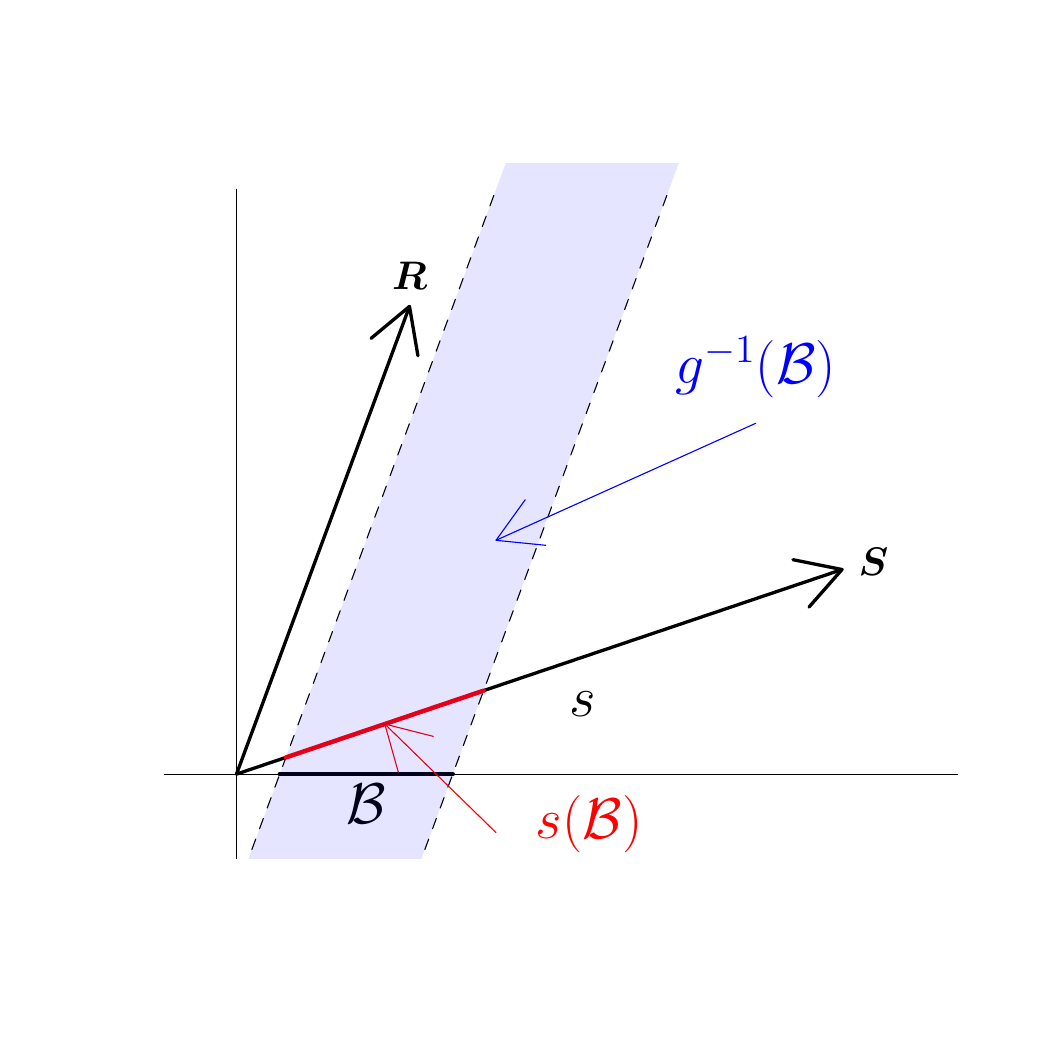
\begin{tikzpicture}[x=1pt,y=1pt]
\definecolor{fillColor}{RGB}{255,255,255}
\path[use as bounding box,fill=fillColor,fill opacity=0.00] (0,0) rectangle (361.35,361.35);
\begin{scope}
\path[clip] ( 49.20, 61.20) rectangle (336.15,312.15);
\definecolor{drawColor}{RGB}{0,0,0}

\path[draw=drawColor,line width= 0.4pt,line join=round,line cap=round] ( 75.46, 49.37) --
	( 75.46,302.86);

\path[draw=drawColor,line width= 0.4pt,line join=round,line cap=round] ( 12.94, 91.62) --
	(361.35, 91.62);

\path[draw=drawColor,line width= 1.2pt,line join=round,line cap=round] ( 75.46, 91.62) -- (294.26,165.55);

\path[draw=drawColor,line width= 1.2pt,line join=round,line cap=round] (282.33,151.98) --
	(294.26,165.55) --
	(276.55,169.10);

\node[text=drawColor,anchor=base west,inner sep=0pt, outer sep=0pt, scale=  1.00] at (300.26,163.26) {{\Large ${\bm S}$}};

\node[text=drawColor,anchor=base,inner sep=0pt, outer sep=0pt, scale=  1.00] at (200.49,112.53) {{\huge $\mathfrak{s}$}};

\path[draw=drawColor,line width= 1.2pt,line join=round,line cap=round] ( 75.46, 91.62) -- (137.97,260.61);

\path[draw=drawColor,line width= 1.2pt,line join=round,line cap=round] (141.02,242.80) --
	(137.97,260.61) --
	(124.07,249.07);

\node[text=drawColor,anchor=base,inner sep=0pt, outer sep=0pt, scale=  1.00] at (137.97,266.61) {{\Large ${\bm R}$}};

\path[draw=drawColor,line width= 0.4pt,dash pattern=on 4pt off 4pt ,line join=round,line cap=round] ( 75.46, 49.37) --
	(169.23,302.86);

\path[draw=drawColor,line width= 0.4pt,dash pattern=on 4pt off 4pt ,line join=round,line cap=round] (137.97, 49.37) --
	(231.75,302.86);

\path[draw=drawColor,line width= 1.6pt,line join=round,line cap=round] ( 91.09, 91.62) --
	(153.60, 91.62);

\node[text=drawColor,anchor=base,inner sep=0pt, outer sep=0pt, scale=  1.00] at (122.34, 73.88) {{\huge $\mathcal{B}$}};
\definecolor{drawColor}{RGB}{255,0,0}

\path[draw=drawColor,line width= 1.6pt,line join=round,line cap=round] ( 93.32, 97.65) --
	(164.77,121.79);
\definecolor{drawColor}{RGB}{0,0,0}

\node[text=drawColor,anchor=base west,inner sep=0pt, outer sep=0pt, scale=  1.00] at (183.63, 68.20) {{\huge $\color{red}{s(\mathcal{B})}$}};
\definecolor{drawColor}{RGB}{255,0,0}

\path[draw=drawColor,line width= 0.4pt,line join=round,line cap=round] (169.23, 70.49) -- (129.04,109.72);

\path[draw=drawColor,line width= 0.4pt,line join=round,line cap=round] (146.55,105.26) --
	(129.04,109.72) --
	(133.93, 92.33);
\definecolor{fillColor}{RGB}{0,0,255}

\path[fill=fillColor,fill opacity=0.10] ( 59.83,  7.12) --
	(122.34,  7.12) --
	(247.38,345.10) --
	(184.86,345.10) --
	cycle;
\definecolor{drawColor}{RGB}{0,0,255}

\node[text=drawColor,anchor=base,inner sep=0pt, outer sep=0pt, scale=  1.00] at (263.01,232.76) {{\huge $\color{blue}{g^{-1}(\mathcal{B}})$}};

\path[draw=drawColor,line width= 0.4pt,line join=round,line cap=round] (263.01,218.36) -- (169.23,176.11);

\path[draw=drawColor,line width= 0.4pt,line join=round,line cap=round] (179.79,190.78) --
	(169.23,176.11) --
	(187.21,174.30);
\end{scope}
\end{tikzpicture}
%\caption{a caption}
%\end{document}

  \end{frame}
  \begin{frame}{Analytically}
  	If we have an unreconciled density the reconciled density can be obtained by linear transformations and marginalisation.
  	\begin{align*}
  	\mbox{Pr}(\tilde{\bm{b}}\in \mathcal{B})&=\mbox{Pr}(\hat{\bm{y}}\in g^{-1}(\mathcal{B}))\\
  	&=\int\limits_{g^{-1}(\mathcal{B})}f(\hat{\bm{y}})d\hat{\bm{y}}\\
  	&=\int\limits_{\mathcal{B}}\int f(\bm{S}\tilde{\bm{b}}+\bm{R}\tilde{\bm{a}})|\left(\bm{S}~\bm{R}\right)|d\tilde{\bm{a}}d\tilde{\bm{b}}
  	\end{align*}
  \end{frame}
  \begin{frame}{Elliptical distributions}
  	Consider case where the base and true predictive distributions are elliptical.
  	\begin{theorem}
  		There exists a matrix $\bm{G}$ such that the true predictive distribution can be recovered by linear reconciliation.
  	\end{theorem}
    This follows from the closure property of elliptical distributions under affine transformations and marginalisation.  
  \end{frame}
%  \begin{frame}{With a sample}
%  	\begin{itemize}
%  		\item Often densities are unavailable but we can simulate a sample from the predictive distribution.
%  		\pause
%  		\item Suppose $\bm{\hat{y}}_{T+h}^{[1]},\ldots,\bm{\hat{y}}_{T+h}^{[J]}$ is a sample from the unreconciled probabilistic forecast.
%  		\pause
%  		\item Then setting $\tilde{\bm y}_{T+h}^{[j]}=\bm{S}\bm{G}\hat{\bm y}_{T+h}^{[j]}$ produces a sample from the reconciled distribution with respect to $g$.
%  	\end{itemize}
%  \end{frame}
  \section{Scoring}
  \begin{frame}{Multivariate Scores}
    \begin{itemize}
    \item Scoring rules can be used to evaluate probabilistic forecasts
        \pause
        \begin{itemize}
	      \item Log Score
	      \item Energy Score
	      \item Variogram score
        \end{itemize}
    \pause
    \item We may want to compare
    \begin{itemize}
    	\item Coherent v Incoherent
    	\item Coherent v Coherent
    \end{itemize}
    \end{itemize}
  \end{frame}
  \begin{frame}{Coherent v Incoherent}
	When using log score
	\begin{theorem}
		Let $f(\bm{y})$ be the true predictive density (on $\mathfrak{s}$) and $LS$ be the (negatively-oriented) log score.  Then there exists an unreconciled density  $\hat{f}(\bm{y})$ on $\mathbb{R}^n$ such that
		\begin{equation*}
		E_{\bm y}\left[LS(\hat{f},\bm{y})\right]<E_{\bm y}\left[LS(f,\bm{y})\right]
		\end{equation*}
	\end{theorem}
    The log score is not proper {\bf in this context}.
  \end{frame}
  \begin{frame}{Simulations}
   	\begin{itemize}
   		\item We have run lots of simulations.
   		\pause
   		\item The main takeaway messages are:
   		    \pause
   		    \begin{itemize}
   		    	\item Reconciliation is better than no reconciliation.
   		    	\pause
   		    	\item Bottom up does not do well.
   		    	\pause
   		    	\item OLS (an orthogonal projection) does reasonably well.
   		    	\pause
   		    	\item MinT (an oblique projection) does best.
   		    \end{itemize} 
   	\end{itemize}
   \hfill\hyperlink{sim}{\beamerbutton{}}
   \end{frame}
   \begin{frame}{Looking ahead}\label{simdisc}
     \begin{itemize}
     	\item The optimal feasible reconciliation method remains an open question even for elliptical distributions.
     	\pause
     	\begin{itemize}
     		\item It is likely to depend on the specific score used.
     	\end{itemize}
        \pause
        \item How should probabilistic reconciliation work for non-elliptical distributions.
        \pause
        \item Are non-linear reconciliation methods worthwhile?
     \end{itemize}	
   \end{frame}
  \begin{frame}
    \Huge{Thank You!}\\
  \pause\Huge{Questions?}
  \end{frame}
  \begin{frame}{GDP}\label{GDP}
  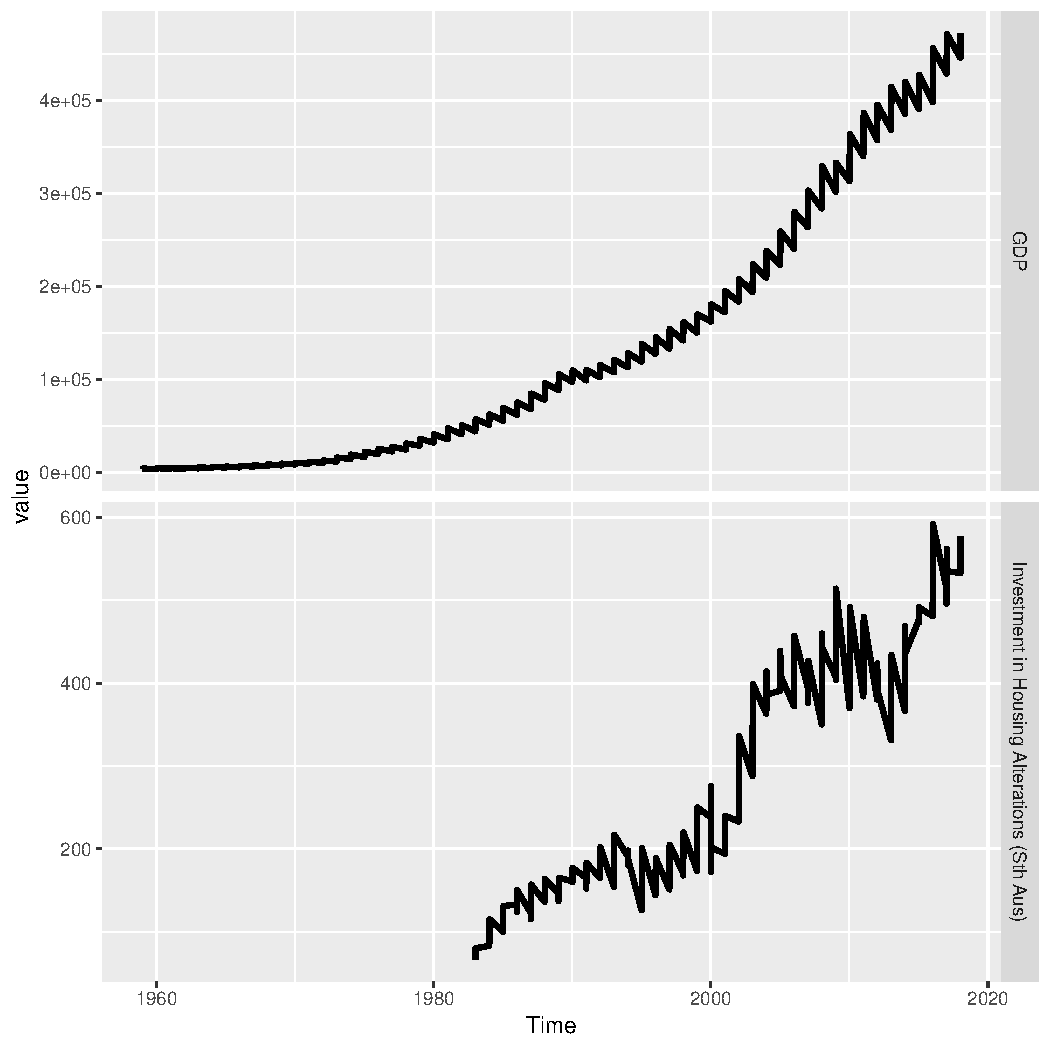
\includegraphics[height=7cm]{Figs/GDP}
  \hyperlink{afterdat}{\beamerbutton{}}
\end{frame}
  \begin{frame}{Aeolos Wind Farm}\label{aelos}
  \centering
  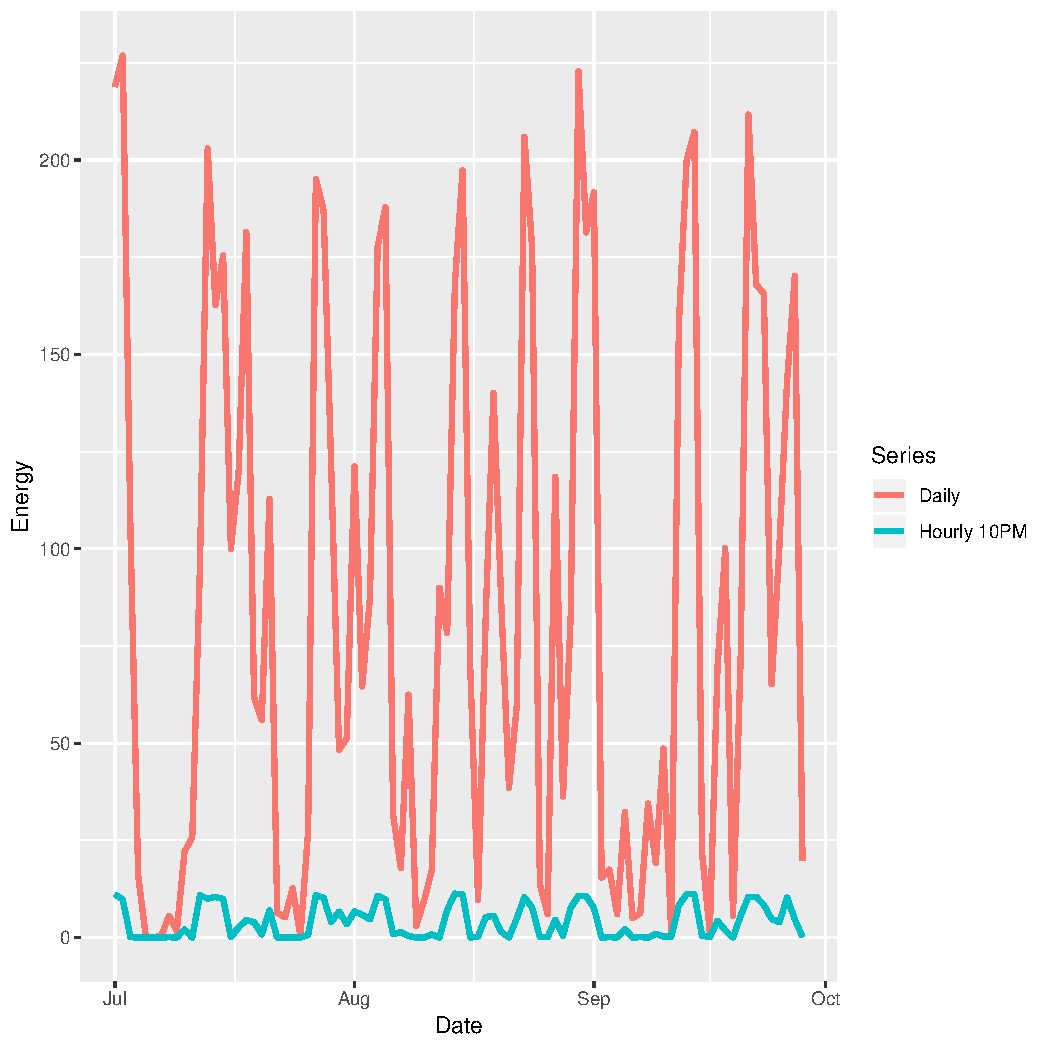
\includegraphics[height=7cm]{Figs/Aeolos_Unscaled}
  \end{frame}
  \begin{frame}{Aeolos Wind Farm}
  \centering
  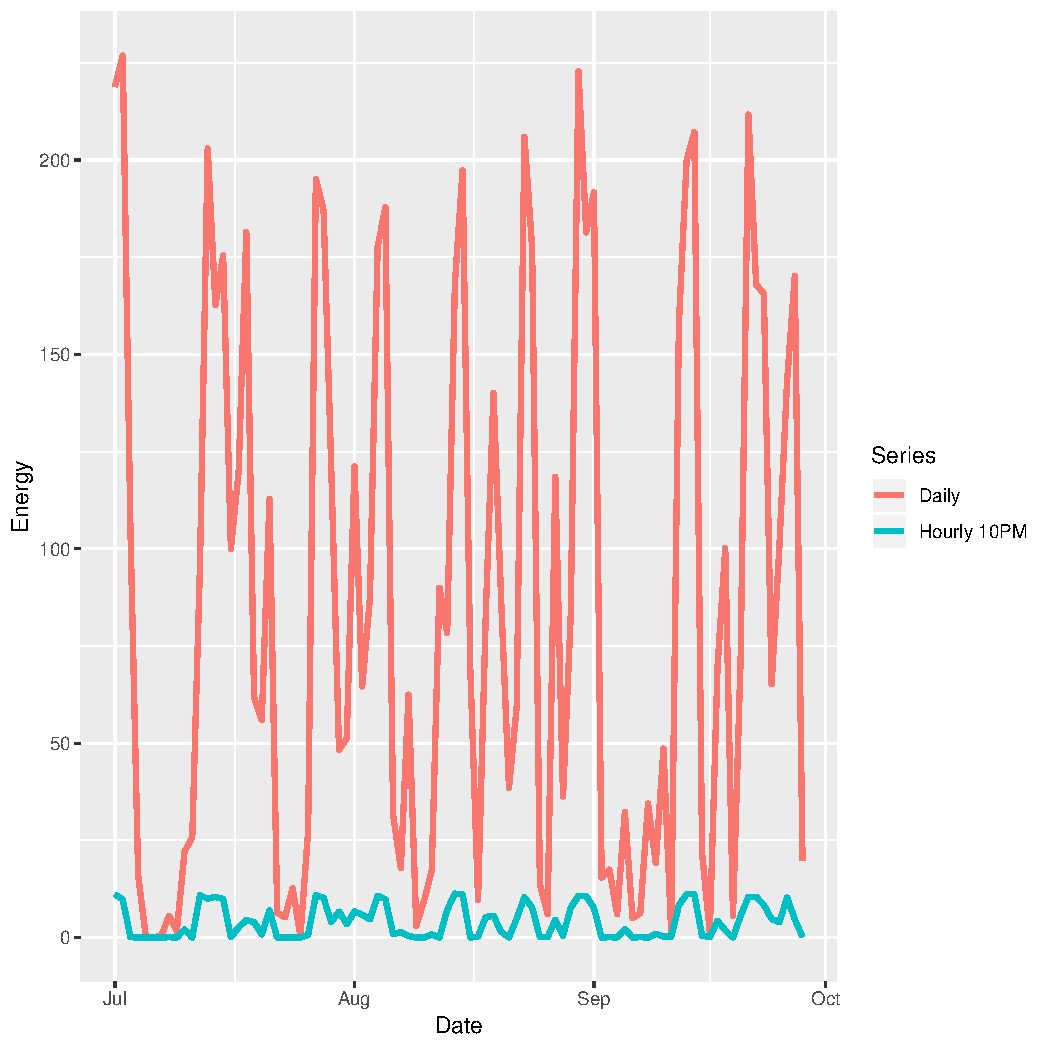
\includegraphics[height=7cm]{Figs/Aeolos_Unscaled}
  \end{frame}
  \begin{frame}{Aeolos Wind Farm}
\centering
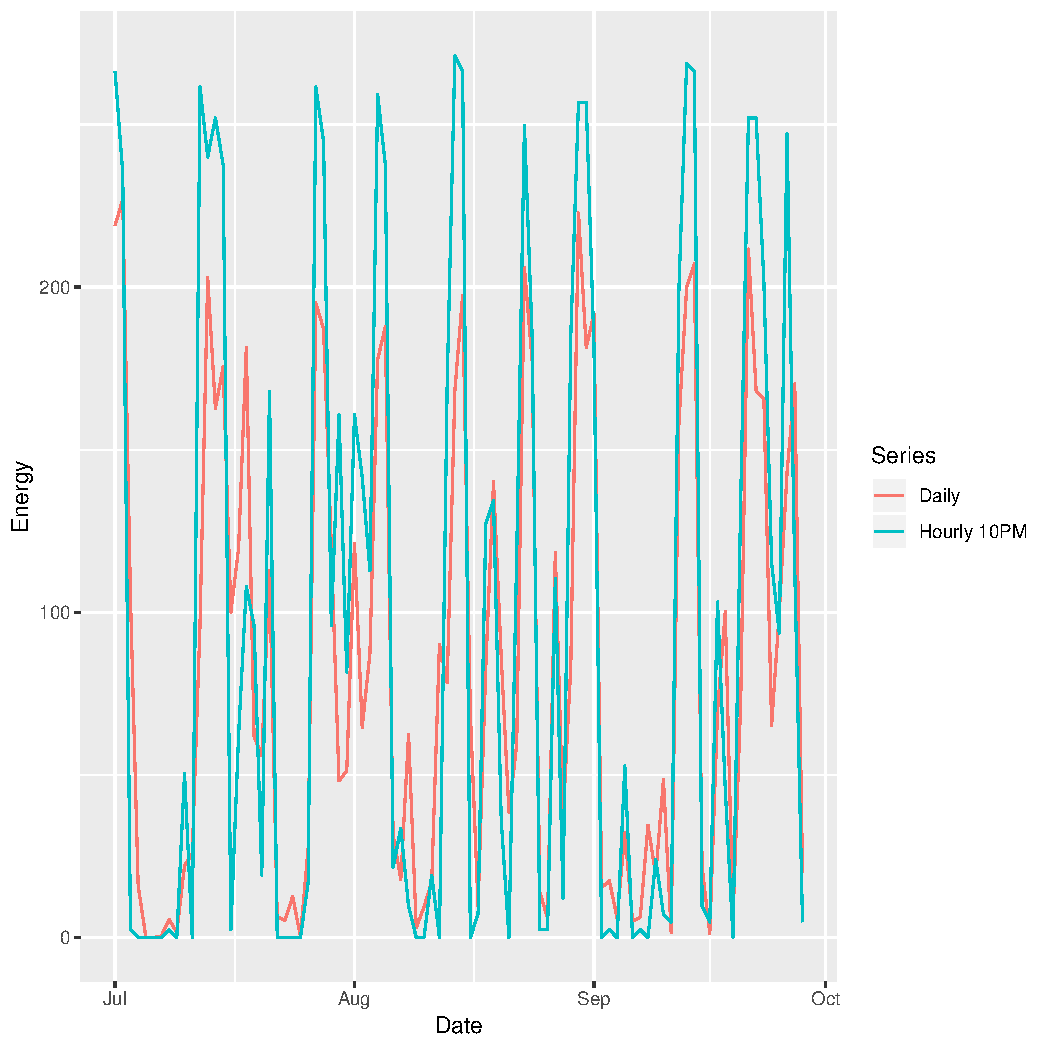
\includegraphics[height=7cm]{Figs/Aeolos_Scaled}
  \hfill\hyperlink{afterdat}{\beamerbutton{}}
\end{frame}
  \begin{frame}{What we do NOT do}\label{bu}
  \begin{itemize}
  	\item Use disaggregate series as predictors (although we can).
  	\item All information is contained in the most disaggregate series.
  	\item In principle using the correct multivariate model for the most disaggregate series and aggregating them should work.
  	\item Disaggregate series are: 
  	\begin{itemize}
  		\item Very noisy
  		\item High-dimensional
  		\item Prone to model misspecification
  	\end{itemize} 
  \end{itemize}
  \hfill\hyperlink{cont}{\beamerbutton{}}
  \end{frame}
  \begin{frame}{Macro Example}\label{macrores}
  Improvement in RMSE of GDP forecasts over seasonal random walk using ARIMA models both without and with reconciliation.
  \begin{table}
  	\begin{center}
  	\begin{tabular}{r|ll}
  	\hline\hline
  	Method & h=1 & h=2  \\
  	\hline
  	Base & 56.1496 & 33.8093\\
  	BU & 54.1873 & 36.1718 \\
  	OLS & 56.6164 & 34.6302\\
  	WLS & 56.6819 & 36.0987\\
  	MinT Sam. &56.2204 & 31.6136 \\
  	MinT Shr. & 57.7249 & 36.8764 \\
  	\hline
  \end{tabular}
  \end{center}
  \end{table}
  	\hfill\hyperlink{cont}{\beamerbutton{}}
  \end{frame}
  \begin{frame}{Simulation Results}\label{sim}
  Hierarchy from earlier bottom series are ARIMA models.  Training sample of 500, one-step ahead forecasts, 1000 replications.
  \begin{table}
  	\centering\small
  	\begin{tabular}{lccc}
  		\toprule
  		Forecasting &{\text{Energy score}} & {\text{Variogram score}} & {\text{Log score}} \\
  		\midrule
  		MinT(Sample) &  {\bf 10.01}   & {\bf 8.41}  & {\bf 11.29} \\
  		OLS          &  10.53   & 8.86  & 11.54 \\
  		Bottom-up    &  12.35   & 9.22  & 12.05 \\
  		Incoherent	 &  11.12   & 9.53  \\
  		\bottomrule
  	\end{tabular}
  \end{table}
\hfill\hyperlink{simdisc}{\beamerbutton{}}
\end{frame}
\end{document}